\documentclass{book}
%\documentclass[8pt]{book}
\usepackage{fancyhdr, flafter, makeidx, float, times}
\usepackage[T1]{fontenc}
\usepackage{graphicx}
\usepackage{fancyvrb}
\usepackage{listings}
\usepackage{varioref}
\usepackage[color]{ods}
\pagestyle{fancy}

%\addtolength{\headwidth}{\marginparsep}
%\addtolength{\headwidth}{\marginparwidth}
%       remember chapter title
%\renewcommand{\chaptermark}[1]%
%                  {\markboth{#1}{}}
%       section number and title
%\renewcommand{\sectionmark}[1]%
%              {\markright{\thesection\ #1}}
%\lhead[\fancyplain{}{\bfseries\thepage}]%
%      {\fancyplain{}{\bfseries\rightmark}}
%\rhead[\fancyplain{}{\bfseries\leftmark}]%
%      {\fancyplain{}{\bfseries\thepage}}
%\cfoot{}

%\setlength{\paperheight}{9in}
%\setlength{\paperwidth}{7.5in}
%\setlength{\textwidth}{5.5in}


%\floatstyle{ruled}
%\newfloat{code}{thp}{lop}[section]
%\floatname{code}{Code}
%\floatstyle{boxed}
%\newfloat{output}{thp}{lop}[section]
%\floatname{output}{Output}


%\DefineVerbatimEnvironment{code}{Verbatim}
%{commandchars=\\\#\?, tabsize=4, xleftmargin=1cm, 
% samepage=false, hfuzz=1pt, fontsize=\small,
% frame=lines, framesep=3mm}
%
%\DefineVerbatimEnvironment{codel}{Verbatim}
%{commandchars=\\\#\?, tabsize=4, xleftmargin=1cm, 
% samepage=false, hfuzz=1pt, fontsize=\small,
% frame=lines, framesep=3mm}

%\newenvironment{fvcode}[2]{\label{#1}
% \Verbatim[commandchars=\~\`\`, tabsize=4, xleftmargin=1cm, 
% samepage=false, hfuzz=1pt, fontsize=\small,
% frame=lines, framesep=3mm, label={Code \ref{#1}: \itshape{#2}}]}{\endVerbatim}

\lstdefinelanguage{tagsets}
 {morekeywords={trigger,do,else,done,if,while,when,break, breakif,
                set,unset,open,close,eval,cmp,exists,any,contains,ODS,proc,run},
  morekeywords=[2]{Define,End,start,finish},
  sensitive=false,
  morecomment=[s]{/*}{*/},
  morestring=[b]",
  morestring=[b]',
 }[keywords,comments,strings,directives]

\lstdefinestyle{tagsetstyle}
 {basicstyle=\small,
  stringstyle=\sffamily,
  keywordstyle=[2]{\bfseries\slshape},
  showspaces=false,
  showstringspaces=false,
  showtabs=false
  emphstyle=\underbar
 }

\lstdefinestyle{HTMLstyle}
 {language=HTML,
  basicstyle=\small,
  stringstyle=\sffamily,
  keywordstyle=[2]{\bfseries\slshape},
  showspaces=false,
  showstringspaces=false,
  showtabs=false
 }

\lstnewenvironment{fvcode}[2]
 {\lstset{label={#1}, caption={#2}, escapechar={~},
          frame=lines, xleftmargin=1cm, style=tagsetstyle}}
 {}

\lstnewenvironment{fvoutput}[2]
 {\lstset{label={#1}, caption={Output: #2}, frame=lines, xleftmargin=1cm, style=HTMLstyle}}
 {}

\lstnewenvironment{sfvcode}
 {\lstset{xleftmargin=1cm, style=tagsetstyle}}
 {}

\lstnewenvironment{sfvoutput}
 {\lstset{xleftmargin=1cm, style=HTMLstyle}}
 {}

\lstnewenvironment{poutput}[2]
 {\lstset{label={#1}, caption={Output: #2}, frame=single, xleftmargin=1cm, style=HTMLstyle}}
 {}

\newenvironment{goutput}[2]{\label{#1} \begin{figure} \caption{#2}}
  {\end{figure}}

\newenvironment{fvhtmcode}[2]{\label{#1}
 \Verbatim[commandchars=\\\{\}, tabsize=4, xleftmargin=1cm, 
 samepage=false, hfuzz=1pt, fontsize=\small,
 frame=lines, framesep=3mm, label={Code \ref{#1}: \itshape{#2}}]}{\endVerbatim}

\newenvironment{fvcodel}[2]{\label{#1}
 \Verbatim[commandchars=\~\`\`, tabsize=4, xleftmargin=1cm, 
 samepage=false, hfuzz=1pt, fontsize=\small,
 numbers=left, numbersep=5pt, 
 frame=lines, framesep=3mm, label={Code \ref{#1}: \itshape{#2}}]}{\endVerbatim}

\newcommand{\commandnames}[1]{\mbox{\large\textbf{#1}}\hfil}
\newcommand{\variablenames}[2]{\mbox{\large\textbf{#2}}\hfil}
\newcommand{\svariablenames}[2]{\mbox{\large\textbf{#2}}\hfil}
\newcommand{\commandargs}[1]{\normalsize\textit{#1}}
\newcommand{\tagsetalias}[1]{\index{#1}\normalsize\textit{Shortcut Alias: #1}}
%\newcommand{\commanditem}[2]{\entry{\commandnames{#1}\commandargs{#2}}}
\newcommand{\commanditem}[2]{\index{#1}\item[\commandnames{#1}]\commandargs{#2}}
\newcommand{\tagsetitem}[2]{\index{#1}\index{#2}\item[\commandnames{#1}]\tagsetalias{#2}}
\newcommand{\stagsetitem}[1]{\index{#1}\item[\commandnames{#1}]}
\newcommand{\variable}[2]{\item[\index{Variables!#1!#2}\variablenames{#1}{#2}]}
\newcommand{\stylevariable}[2]{\index{Variables!Style!#1!#2}\item[\svariablenames{#1}{#2}]}
\newenvironment{entry}
     {\begin{list}{}%
         {\renewcommand{\makelabel}{\commandnames}%
            \setlength{\labelwidth}{35pt}%
            \setlength{\leftmargin}{\labelwidth+\labelsep}%
         }%
     }%
     {\end{list}}


%\newenvironment{sfvcode}{
% \Verbatim[commandchars=\~\`\`, tabsize=4, xleftmargin=1cm, 
% samepage=false, hfuzz=1pt, fontsize=\small,
% frame=lines, framesep=3mm]}{\endVerbatim}

%\newenvironment{fvoutput}[2]{\label{#1}
% \Verbatim[commandchars=\~\`\`, tabsize=4, xleftmargin=1cm, 
% samepage=false, hfuzz=1pt, fontsize=\small,
% frame=lines, framesep=3mm, label={Output \ref{#1}: \itshape{#2}}]}{\endVerbatim}

%\newenvironment{sfvoutput}{
%\Verbatim[commandchars=\~\`\`, tabsize=4, xleftmargin=1cm, 
%samepage=false, hfuzz=1pt, fontsize=\small,
%frame=lines, framesep=3mm, label={\itshape Output}]}{\endVerbatim}

\newcounter{calloutcounter}[chapter]
\setcounter{calloutcounter}{1}
\newcommand{\calloutref}[1]{{\bfseries\ref{#1}}}
\newcommand{\callout}[1]{\label{#1}
 \refstepcounter{calloutcounter}
 \hspace{-5pt}
 {\bfseries 
  \thecalloutcounter
 \hspace{5pt}}
}

%  \marginpar[\flushright{\bfseries\value{calloutcounter}$\longrightarrow$}]
%             {{\bfseries $\longleftarrow$\value{calloutcounter}}}}

\newcommand{\calloutRepeat}{
 \hspace{-5pt}{\bfseries 
 \thecalloutcounter\hspace{5pt}}
}

%  \marginpar[\flushright{\bfseries\value{calloutcounter}$\longrightarrow$}]
%             {\bfseries$\longleftarrow$\value{calloutcounter}}}
% \hspace{-5pt}{\bfseries \value{calloutcounter}\hspace{0pt}}

\makeindex

%\includeonly{introduction, chapter1, chapter2,chapter3, chapter6, chapter7a, chapter4, chapter5, chapter5a, chapter4a, chapter7,chapter8,chapter9}

\begin{document}
\lstset{language=tagsets}
%\lstset{language=SAS}

% The way the preface titles are to be
\fancyhead{} %clear all fields
\fancyhead[LO,RE]{\thepage}
\fancyhead[RO]{}
\fancyhead[LE]{}
\fancyfoot[CO,CE]{}

\frontmatter
\title{ODS Markup: \\
Tagsets by Example}
\author{Eric Gebhart\\
SAS Institute}
\renewcommand{\today}{September 22, 2003}
\pagenumbering{roman}
\maketitle
  \section*{Preface}
\include{preface}
\cleardoublepage
\tableofcontents
\cleardoublepage
%\listoflistings
\cleardoublepage
\listoftables

%\listof{code}
%\listof{output}
% -----------------------document body

\mainmatter
\cleardoublepage
\pagenumbering{arabic}
\fancyhead{} %clear all fields
%\setlength{\headrulewidth}{1pt}
\lhead[\rm\thepage]{\sl\rightmark}
\rhead[\sl\leftmark]{\rm\thepage}

%The old fancyhead way.
%\fancyhead[LE,RO]{\thepage}
%\fancyhead[RE]{\bfseries Chapter \thechapter. \chaptermark}
%\fancyhead[LO]{\bfseries Section \thesection \sectionmark}
%\fancyfoot[CO,CE]{}

\part{Using ODS Markup and Tagsets}
%{
%These chapters will cover the basics of the ods markup statement,
%proc template, and tagsets.  The most commonly used tagsets will
% be explored and used.
%}

\cleardoublepage
\chapter{Introduction}
ODS markup and tagsets are the best way to create markup output
from SAS.  This book is divided into sections that will enable
you to get the most out of ODS Markup and Tagsets.  The first
section shows how ODS Markup and Tagsets are used.  Using an
ODS destination that is defined by a tagset is no harder than
using any other destination.  The most popular ODS Markup 
destinations are covered in this first section.

The next sections dig deeper into how Tagsets work and what
you can do to modify them or create your own.  This may
seem daunting at first, but frequently it is quite easy to
get Tagsets to do exactly what you want, saving lots of time
and effort further down a project's path.


\cleardoublepage
\chapter{The basics}
This chapter will cover the basics of using ODS Markup family of destinations.
There are a lot of ODS destinations in this family, and they are ready to
use.  By the end of this chapter you will have some idea of the destinations 
available, and how to use them.

ODS Markup is just another ODS destination that works very much
like every other ODS destination.  It was originally derived from
the original ODS HTML destination, so if you are familiar with ODS HTML,
then you are already very familiar with ODS Markup.

The way ODS Markup differs is that we will almost never use ODS Markup as
a destination name.  ODS Markup should be thought of as a family of destinations.
These destinations are defined using a type of template called Tagsets.  Each
Tagset definition is a new ODS destination.
 
The good news is that there are already a lot of Tagsets defined, so all we need
to do is use them.  Since Tagsets define destinations within the ODS Markup family
the only thing we really need to know is their names.  Once we know the tagset's 
name we know the destination name, and we can easily construct an ODS statement
that will use that ODS destination.



\section{It's all in the Name}
\index{basics}
\index{proc template}
\index{itemstore}
\index{sasuser}
\index{sashelp}
A tagset is a SAS program that uses Proc Template.  There are a lot of advantages to
this.  It means that SAS can update a tagset, make a fix, and even email that tagset
to anyone that wants it.  Updates to the Tagsets that shipped with SAS are available
for download on the Support.sas.com website.  Frequently there are also additional 
tagsets that were not shipped with SAS.  Another benefit, is that if you want to learn
to program Tagsets, you can create your own, or modify the Tagsets provided by SAS.

For now, the most important thing to know, is what are the Tagsets available, and 
what are they named.  All we really need is their names.  But where do we look?
When a Tagset is run in SAS, Proc Template compiles the Tagset and stores it
When a Tagset is run in SAS, Proc Template the Tagset
it into a binary format which is then stored on disk in an itemstore.
Typically this file will be in sasuser.  But can be placed anywhere
using the 'ODS path' statement.  If administrative priviledges are
available the template can be put in SASHELP where it will be
available to all users on the system.  Once a template is compiled
there is no need to compile it again unless it's itemstore is
deleted.  All Tagsets that ship with SAS are in SASHELP.

Thankfully, Proc Template handles all of this for us, and will look for Tagsets
in all the right places.  All we need is 3 lines of SAS code, and we will have
all the names for all the Tagsets.


\subsection{The tagset directory}
Templates are kept in directories within the itemstore.  ODS will automatically look for 
tagsets in the tagsets directory.  The following example shows how to get a list
of tagsets, and the output it generates.

\begin{fvcode}{list_tagsets}{Simple ODS Markup Statement}
       proc template;
           list tagsets;

                               The SAS System                               1
                                                  13:00 Monday, August 7, 2006

                Listing of: SASHELP.TMPLMST
                Path Filter is: Tagsets
                Sort by: PATH/ASCENDING
 
                Obs    Path                             Type
                 1     Tagsets                          Dir   
                 2     Tagsets.Cascading_stylesheet     Tagset
                 3     Tagsets.Chtml                    Tagset
                 4     Tagsets.Colorlatex               Tagset
                 5     Tagsets.Config_debug             Tagset
                 6     Tagsets.Csv                      Tagset
                 7     Tagsets.Csvall                   Tagset
                 8     Tagsets.Csvbyline                Tagset
                 9     Tagsets.Default                  Tagset
                10     Tagsets.Docbook                  Tagset
                11     Tagsets.Event_map                Tagset
                12     Tagsets.ExcelXP                  Tagset
                13     Tagsets.Graph_rtf                Tagset
                14     Tagsets.Html4                    Tagset
                15     Tagsets.Htmlcss                  Tagset
                16     Tagsets.Htmlpanel                Tagset
                17     Tagsets.Imode                    Tagset
                18     Tagsets.Latex                    Tagset
                19     Tagsets.MSOffice2k               Tagset
                20     Tagsets.Mlatex                   Tagset
                21     Tagsets.Mvshtml                  Tagset
                22     Tagsets.Namedhtml                Tagset
                23     Tagsets.Odsapp                   Tagset
                24     Tagsets.Odsgraph                 Tagset
                25     Tagsets.Odsstyle                 Tagset
                26     Tagsets.Odsxrpcs                 Tagset
                27     Tagsets.OpenOffice_rtf           Tagset
                28     Tagsets.Phtml                    Tagset
                29     Tagsets.Pyx                      Tagset
                30     Tagsets.Rtf                      Tagset
                31     Tagsets.Rtf_sample               Tagset
                32     Tagsets.SASReport11              Tagset
                33     Tagsets.SASReport12              Tagset
                34     Tagsets.SASReport13              Tagset
                35     Tagsets.SASReport14              Tagset
                36     Tagsets.SASReport15              Tagset
                37     Tagsets.SASReport_html           Tagset
                38     Tagsets.SASReport_html1          Tagset
                39     Tagsets.Sasreport_html11         Tagset
                40     Tagsets.Short_map                Tagset
                41     Tagsets.Simplelatex              Tagset
                42     Tagsets.Style_display            Tagset
                43     Tagsets.Style_popup              Tagset
                44     Tagsets.Supermap                 Tagset
                45     Tagsets.Tablesonlylatex          Tagset
                46     Tagsets.Text_map                 Tagset
                47     Tagsets.Tpl_style_list           Tagset
                48     Tagsets.Tpl_style_map            Tagset
                49     Tagsets.Troff                    Tagset
                50     Tagsets.Wml                      Tagset
                51     Tagsets.Wmlolist                 Tagset
                52     Tagsets.Xbrl                     Tagset
                53     Tagsets.Xhtml                    Tagset
       run;

NOTE: PROCEDURE TEMPLATE used (Total process time):
      real time           1:40.15
      cpu time            0.28 seconds
      
\end{fvcode}

\section{Using a tagset}
That is a lot of Tagsets!  For now, lets concentrate on the obvious
ones.  
To use a tagset, all that is needed is the proper ods statement.
ODS Markup is not all that different from ODS HTML, in fact, ODS
Markup can do everything ODS HTML can, plus a little more.
The simplest form of the ODS Markup statement is shown 
in Figure \ref{ods_markup_stmt} on page \pageref{ods_markup_stmt}.

\index{ods statement}
\begin{fvcode}{ods_markup_stmt}{Simple ODS Markup Statement}
   
    ods markup file='test.xml';

    ....

    ods markup close;

\end{fvcode}

\index{ods markup statement}
\index{tagsets.default}

The result of those statements will be the creation of the 'test.xml' output
file.  The output of that file will have a format as defined by the default
tagset, which is named, tagsets.default.

But there are other ways to specify an ODS statement that accomplish the same thing.
Figure \ref{ods_markup_stmt_perm} on page \pageref{ods_markup_stmt_perm}.
shows ods statements which are equivalent with one exception.

\begin{fvcode}{ods_markup_stmt_perm}{ODS Markup Statement Permutations}
\index{ods markup statement!permutations}

    ods markup file='test.xml';

    ods markup tagset=default file='test2.xml';

    ods tagsets.default file='test3.xml';

\end{fvcode}

The exception is the third statement.  That statement is different because the destination
name is no longer markup.  The destination name is tagsets.default.   Because it has a
unique name it can run simultaneously with ods markup.  Just like ODS RTF can run simultaneously
with ODS HTML.  The first two statements cannot be used simultaneously because they have the
same destination name.  The second ODS Markup 
statement would automatically close the first one.  This happens because ODS destination names
must be unique.  There is a way around that, using ODS' ID syntax, but that belongs in another
book.  Beside's that syntax is mostly uneccessary if we use the tagset name as the destination
name, and the resulting code is more readable and concise.


As of SAS 9.1, ODS HTML is also a tagset.  Which means ODS HTML is really ODS Markup.  Consider
the statements in figure \ref{ods_markup_stmt_perm2} on page \pageref{ods_markup_stmt_perm2}.

\index{ods markup statement!permutations}
\begin{fvcode}{ods_markup_stmt_perm2}{ODS Markup Statement Permutations}
    ods html file='test1.html';

    ods html4 file='test2.html';

    ods tagsets.html4 file='test3.html';

    ods markup tagset=html4 file='test4.html'
\end{fvcode}

Each one of those statements is roughly equivalent.  All of them use the html4 tagset.  So
the markup each of them creates will be the same.  But each ODS statement creates a unique
output destination.  They can all run simultaneously without conflict.  They can all have their
own select or exclude statements and be opened or closed at different times.   

There is one thing that makes html special.  Normally a tagset cannot be referenced by
it's simple name unless the tagset option is used. But there are a few special tagsets that
can be referenced as if they are a simple ODS destination.  
Table \ref{shortcut_destinations} on page \pageref{shortcut_destinations} shows the list
of shortcut names and their descriptions.


\index{Simple names}
\index{Shortcut destinations}
\begin{table}\caption{Shortcut Destination names}
\label{shortcut_destinations}
\begin{tabular}{l|l}
%\multicolumn{2}{c}{Shortcut Destinations} \\ 
\hline
HTML &  Alias for HTML4 \\
HTML4 & 4.0 compliant HTML with concessions for browser compatibility. \\
PHTML & Plain HTML.  Simple stylesheet, simple HTML. \\
HTMLCSS & 4.0 compliant HTML with fewer concessions. \\
CSV &  Comma separated values.  Tables only. \\
CSVAll & CSV with titles, bylines, notes, etc. \\
CSVByline & CSV with bylines only. \\
WML &  Wireless Markup Language. - No longer in vogue. \\
CHTML & Compact HTML. Very simple HTML with no styles. \\
LaTeX & LaTeX output with style and color support. \\
Troff & troff output which is very simple. \\
MSOffice2K & HTML for importing into Word and Excel. \\
Imode & Compact HTML that has no table tags.  Used extensively in Japan. \\
DocBook &  XML format for documents. \\
SasReport & XML format used internally by other SAS products.
\end{tabular}
\end{table}

While these are special, the custom tagsets that can be written are no less special.  These
custom tagsets cannot be referenced by their simple names but they will be output destinations just
as these are.  Because Markup is a single destination, the prefered way to use tagsets is to
use their two part name.  There is a trend away from using these shortcut names, so most of the
newer tagsets like ExcelXP and RTF can only be referenced by their full name.
See Figure \ref{ods_markup_stmt_active} on page \pageref{ods_markup_stmt_active} shows the list

\index{ods markup statement!permutations}
\index{ods markup statement!Multiple Active}
\begin{fvcode}{ods_markup_stmt_active}{Multiple Active Markup Destinations}

    ods tagsets.ExcelXP file='test.xml';
    ods tagsets.RTF file='test.rtf';

    proc print data=sashelp.class; 
    run;

    ods tagsets.ExcelXP close;
    ods tagsets.RTF close;

\end{fvcode}
     
\section{Summary}
Using ODS Markup does not have to be complicated or difficult, all we really
need is the name of the Tagset, and we can use them just like any other destination.
Finding their names is very simple Proc Template code, and adding an ods statement that uses them is
just as easy.  It won't hurt anything to try out a destination just to see what it
will create.  Go ahead, play, try them out.  The next chapters will go into more 
detail for many of the more popular and useful Tagsets that are available.

The most confusing thing about the ods markup statement is that it
is almost never used by it's name.  Aside from that it is almost
the same as any other ods destination, especially the ODS HTML
destination in previous releases of SAS.


\cleardoublepage
\chapter{Using The CSV Destinations.}
The CSV Tagsets are some of the most useful tagsets around,
the format has been used for decades by various applications
and everyone knows what to expect from a CSV file.  This chapter
will explain how to use the 3 different CSV tagsets provided by SAS.

\index{CSV}
\index{Excel!CSV}
\index{Excel!Live Data}
Comma separated values are one of the simplest formats that are
is understood by many different applications.  The disadvantage is that
there is no formatting, fonts, or colors.  Still CSV files work
very well for many applications.  A CSV file can be connected as
live data to an Excel Template.  This can be a convenient way to
publish Excel spreadsheets to many people.  

\index{CSV|Tagsets}
\index{CSV|CSVALL}
\index{CSV|CSVBYLINE}
There are three different CSV Tagsets shipped with SAS.  The
simplest is the CSV Tagset, next comes CSVByline, and last
is CSVAll.  The CSV Tagset only creates output from tabular
data, there are no titles, footnotes, bylines, Notes, there
is nothing but tables.  It didn't take long to find out that
there were people who wanted titles and footnotes and everything
else, that's when CSVAll came into existence.  It also became
apparent that just having tables and bylines was a nice thing to
have, so CSVBylines was born.  All of these tagsets use the same
base Tagset to create the CSV data, so there is no other difference
in behavior besides the verbosity of the output.

Both CSV and CSVAll have aliases so that they can be referenced by
a simple name, rather than the full tagset name.  CSVByline has no
alias, so it must be used with it's full name.  Here are examples
of each of these ODS statements.

\begin{sfvcode}
ODS CSV file='test.csv';
ODS CSVAll file='testall.csv';
ODS tagsets.CSVByline file='testby.csv';
\end{sfvcode}

Using these statements around a simple Proc Print will show how
these destinations vary.

\begin{sfvcode}
ODS CSV file='test.csv';
ODS CSVAll file='testall.csv';
ODS tagsets.CSVByline file='testby.csv';

options obs=6;

proc sort data=sashelp.class out=sorted;
     by sex;

Proc print data=sorted;
     by sex;
run;

ODS _all_ close;
\end{sfvcode}

None of the output from this example is very complicated,
but each has it's differences.  The CSV Tagset ignores the title
and the bylines. But it does create the two tables as a result of
the by.

\begin{sfvoutput}
"Obs","Name","Age","Height","Weight"
"1","Alice",13,56.5,84.0
"2","Barbara",13,65.3,98.0
"3","Carol",14,62.8,102.5

"Obs","Name","Age","Height","Weight"
"4","Alfred",14,69.0,112.5
"5","Henry",14,63.5,102.5
"6","James",12,57.3,83.0
\end{sfvoutput}

The CSVByline Tagset adds the bylines, but nothing else.

\begin{sfvoutput}
"Sex=F"
"Obs","Name","Age","Height","Weight"
"1","Alice",13,56.5,84.0
"2","Barbara",13,65.3,98.0
"3","Carol",14,62.8,102.5

"Sex=M"
"Obs","Name","Age","Height","Weight"
"4","Alfred",14,69.0,112.5
"5","Henry",14,63.5,102.5
"6","James",12,57.3,83.0
\end{sfvoutput}

Finally, the CSVAll tagset adds in the title.  If there were
footnotes, or procedure titles, or any of the four flavors of
notes; Note, Warning, Error, or Fatal, those would be included as well.

\begin{sfvoutput}
The SAS System

"Sex=F"
"Obs","Name","Age","Height","Weight"
"1","Alice",13,56.5,84.0
"2","Barbara",13,65.3,98.0
"3","Carol",14,62.8,102.5

"Sex=M"
"Obs","Name","Age","Height","Weight"
"4","Alfred",14,69.0,112.5
"5","Henry",14,63.5,102.5
"6","James",12,57.3,83.0
\end{sfvoutput}

In the beginning it seemed that this was everything that any CSV tagset
would ever need to do.  But even the simplest of outputs is not always 
that simple.  Tagsets needed to be able to adapt to what was needed of them.
The best way to do that is to have the ability to give the tagset some variable
to help it make decisions on how to behave.  Up until SAS 9.1.3 the only way
to do that was with macro variables.  Macro variables still work, but now there
is a better way.  With SAS 9.1.3 the ODS Markup statement was given a new option,
the options(...) option.  Options are a nearly arbitrary set of key value pairs
that the tagset will recieve.  It is completely up to the Tagset to process those
values and use them. 

Surprisingly the CSV Tagset has quite a number of options. In fact everything
that the CSVAll and CSVByline tagsets do can be done by the base CSV Tagset.
In SAS 9.1.3 the only thing CSVALL and CSVByline Tagsets do is set up some new defaults for
the CSV options available.

With the proliferation of Tagset options it didn't take long to figure out we needed
another option, Help!  All Tagsets that have options have an option called doc.  The Doc
option is all you need to find out just what a Tagset can do.  Asking for help may be
the first thing you want to do when using a new tagset.  If there are options, Help will
tell you about them.  Help isn't in all of the Tagsets, but the number is growing and
it never hurts to ask.  Here is how we ask for help.

\begin{sfvcode}
ODS CSV file='test.csv' options(doc='help');
\end{sfvcode}

The output from help will go to the log and for CSV, it looks like this.

\begin{sfvoutput}
==============================================================================
The CSV Tagset Help Text.
 
This Tagset/Destination creates output in comma separated value format.
 
Numbers, Currency and percentages are correctly detected and show as numeric values.
Dollar signs, commas and percentages are stripped from numeric values by default.
 
==============================================================================
 
These are the options supported by this tagset.
 
Sample usage:
 
ods csv options(doc='Quick'); 
 
ods csv options(currency_as_number='yes' percentage_as_number='yes' delimiter=';'); 
 
Doc:  No default value.
     Help: Displays introductory text and options.
     Quick: Displays available options.
 
Delimiter:   Default Value ','
     Sets the delimiter for the values.  Comma is the default.  Semi-colon is
     a popular setting for european sites.
 
currency_as_number:   Default Value 'No'
     If 'Yes' currency values will not be quoted.
     The currency values are stripped of punctuation and currency symbols
     so they can be used as a number.
 
percentage\_as\_number:   Default Value 'No'
     If 'Yes' percentage values will not be quoted.
     The percentages are stripped of punctuation and the percent sign
     so they can be used as a number.
 
Currency\_symbol:   Default Value '\$'
     Used for detection of currency formats and for 
     removing those symbols so excel will like them.
     Will be deprecated in a future release when it is
     no longer needed.        
 
Decimal\_separator:   Default Value '.'
     The character used for the decimal point.
     Will be deprecated in a future release when it is no longer needed.
 
Prepend\_Equals:   Default Value 'no'
     Put an equal sign in front of quoted number values.
     This only works in conjunction with quote_by_type.
 
quote\_by\_type:   Default Value 'no'
     Put values based on the type, not based on what the regex match for number.
 
Table\_Headers:   Default Value 'yes'
     If no, skip the header section of all tables.
 
Thousands\_separator:   Default Value ','
     The character used for indicating thousands in numeric values.
     Used for removing those symbols from numerics so excel will like them.
     Will be deprecated in a future release when it is no longer needed.
 
Quoted\_columns:   Default Value ''
     A list of column numbers that indicate which values should be quoted
     ie. Quoted\_columns="123"
 
Empty\_Missing:   Default Value 'no'
     If yes, missing values will not show in any way other than positionally.
 
Bylines:   Default Value: No
     If yes bylines will be printed
 
Titles:   Default Value: No
     If yes titles and footnotes will be printed
 
Notes:   Default Value: No
     If yes Note, Warning, Error, and Fatal notes will be printed
 
Proc\_Titles:   Default Value: No
     If yes titles generated by the procedures will be printed
 
\end{sfvoutput}


The help you get will depend upon which version of the tagset you have.
There are the expected options that reflect the behaviors we have seen
from the CSVAll and CSVByline Tagsets, but there is much more.  One
of the most used options is Delimiter, this makes it easy to change the
field delimiter to a ;, a | or even tabs.  Another thing that became
obvious was that there needed to be a way to detect numbers in any one
of the various European formats.  That's where decimal\_separator, thousands\_separator
and currency\_symbol come in.  Not everyone uses a '.' for decimals, or ',' for
thousands. 

There are a few less obvious options in there.  Table\_headers turns the table\_headers
on and off.  Empty\_missing makes missing values go completely away, with just it's
field delimiters showing where it would have been.  

Currency\_as\_Number, and Percentage\_as\_Number,
are there because not everyone wants those values as strings, So if you want them as numbers,
these options will do that for you, they will also strip out any symbols that would prevent
Excel from seeing those values as numbers.

Another option that is just for excel, is prepend\_equals, this option will put an '=' in front
of quoted numbers so that Excel will read the value correctly, even if it has leading zeros.  So
if you have leading zero's this is the option you want.

The last two have to do with quoting.  Currently, the CSV tagset tries it's best to figure out
what is a string and what is a number.  It doesn't always do exactly what we want.  Part of
the problem is that some procedures don't tell the Tagset what is what.  Proc Print is one of
those procedures that does say which value is a string and which is a number.  The quote\_by\_type
option tells the tagset to stop guessing and do what Proc Print or any other proc says.  The
exception to this, until SAS 9.2, is Proc Report, and Proc Tabulate.  Those are the two Procs
that don't give the tagset any clues.

To further extend the ability to control quoting, There is a Quoted\_columns option that will
allow for columns to be specified by number.  So if all else fails and you still can't get
your values quoted where you want, this option should do the trick.


By default the csv tagset only displays tables.  Turning on bylines so that it looks
like the output from the CSVByline Tagset 
is just a matter of setting the bylines option to yes.  Changing the Delimiter to a
';' is just as easy.  Of course we could have used the CSVByline Tagset with just
the delimiter option to do the same thing.

\begin{sfvcode}
ODS CSV file='test.csv' options(delimiter=';' bylines='yes');
ODS tagsets.CSVByline file='test.csv' options(delimiter=';');

options obs=6;

proc sort data=sashelp.class out=sorted;
     by sex;

Proc print data=sorted;
     by sex;
run;

ODS _all_ close;
\end{sfvcode}

The output from both of these ODS statements looks identical.

\begin{sfvoutput}
"Sex=F"
"Obs";"Name";"Age";"Height";"Weight"
"1";"Alice";13;56.5;84.0
"2";"Barbara";13;65.3;98.0
"3";"Carol";14;62.8;102.5

"Sex=M"
"Obs";"Name";"Age";"Height";"Weight"
"4";"Alfred";14;69.0;112.5
"5";"Henry";14;63.5;102.5
"6";"James";12;57.3;83.0
\end{sfvoutput}

Knowing how the CSVByline and CSVAll Tagsets work can be quite handy, Especially
if you find that you always want the same basic set of options.  It is much easier
to create your own Tagset than it is to always type in the same options over and over.
Here is the entire code for the CSVByline Tagset.  Before you look, realize that most
of this is copied and pasted from the CSV Tagset.

\begin{sfvcode}
   define tagset tagsets.csvbyline;
       parent=tagsets.csv;

        define event initialize;
            set \$options['BYLINES'] 'yes';
            trigger set_options;
            trigger documentation;
            trigger compile_regexp;
        end;
    end;
\end{sfvcode}

The only addition to the copied and pasted code is this line.

\begin{sfvcode}
            set \$options['BYLINES'] 'yes';
\end{sfvcode}

We can take advantage of this knowledge and create our own CSV Tagset that
has it's own set of default option values.  If we want the same behavior from
the new Tagset as 
our previous example a new name is probably in order.  After all it's no longer
comma separted values, it's semi-colon separated values. 
Our new Tagset would look like this.  Be aware that option
names are always capitalized inside the tagset.

\begin{sfvcode}
proc template;
   define tagset tagsets.ssvbyline;
       parent=tagsets.csv;

        define event initialize;
            set \$options['BYLINES'] 'yes';
            set \$options['DELIMITER'] ';';
            trigger set_options;
            trigger documentation;
            trigger compile_regexp;
        end;
    end;
run;
\end{sfvcode}

All we have to do is run that Proc Template, and our new tagset is ready to use.
Congratulations! You've just written your first Tagset!  If someone else wants 
output that has bylines and semi-colons for field separators, just tell them to
do this!

\begin{sfvcode}
     ODS tagsets.ssvbyline file='test.csv' options(doc='help');
\end{sfvcode}

The output looks exactly like the output above.  It is, after all, generated the same way.

\section{Summary}
The CSV destinations are very easy to use and although the output is very simple, there are
many options that can be used to control how that output is created.  ODS Markup options 
provide a very versatile way to change the behavior of any Tagset destination.  Finding out
what those options are, and how to use them is as easy as asking for help.  Add options(doc='help')
to any ODS Markup/tagsets statement and find out just what that Tagset can do for you.
Creating a new Tagset that sets the options just the way you want is almost as easy is copy
and paste.    
That's what tagsets are all about, creating output just the way you want it,
in a reusable and easy way.







\cleardoublepage
\include{chapter15}
\cleardoublepage
\chapter{Using LaTeX}
Besides HTML and XML, LaTeX output is one of the most useful
and versatile output destinations available.  LaTeX is commonly
used in publishing and is capable of creating several viewable
formats, including PDF and Postscript.  LaTeX supports color
and various image formats.
Sadly, this destination is largely overlooked.
This chapter will discuss how to use it to advantage. 

\section{The LaTeX statement}
\index{ODS Statements!Latex}
Latex is one of the special destination names that is 
shorthand for tagsets.latex.  But there are other latex
tagsets.  Color\_latex differs only in the way it invokes the
usepackage statement to include the 'stylesheet' generated by
latex.  Simple\_latex is the most simplistic form of latex which
lends itself to embedding in other LaTeX documents.

The best way to use the latex tagsets is with an external stylesheet.
Using an external stylesheet is the only way to turn color on.  The
stylesheet includes usepackage statements for all the packages needed
to render the latex.  It also defines macros for the styles and formatting.

Another requirements of using latex is that a url without the .sty extension
be specified for the stylesheet.  This is the name that will go in the 
usepackage statement in the preamble of the latex document.
A sample ods latex statement is shown here.

\begin{sfvcode}
        ods latex file="test.tex" stylesheet="test.sty"(url="test");
\end{sfvcode}

\subsection{Color Support}
\index{Latex!Color}
\index{Tagsets!Color\_Latex}
Color LaTeX is really the same as the regular latex tagset.
The only difference is that a flag is set so that colors will
be used.  The entire tagset looks like this.  The change is
the addition of the color option.

\begin{sfvcode}
    define tagset tagsets.colorlatex; 
        parent=tagsets.latex;

        define event stylesheet_link;
            put CR '\usepackage[color]{';
            put URL;
            put '}' CR CR;
        end;

    end;
\end{sfvcode}

A better color latex tagset would work without a stylesheet url
being specified on the ods statement.  This is only possible in
SAS 9.1, but is a perfect example of how useful data step functions
can be.

\begin{sfvcode}
proc template;
    define tagset tagsets.colorlatex; 
        parent=tagsets.latex;

        define event stylesheet_link;
            put CR '\usepackage[color]{';
            put scan(url, 1, '.');
            put '}' CR CR;
        end;

    end;
run;

ods tagsets.colorlatex file="test.tex" stylesheet="test.sty";
proc print data=sashelp.class;run;
ods _all_ close;
\end{sfvcode}

\section{Compiling the LaTeX Output}
There is no browser for LaTeX.  LaTeX must be compiled into the 
document type desired.  Different commands create the various forms
of browseable output.

\subsection{The latex Command}
\index{Latex}
\index{Latex!Compiling}
\index{Latex!DVI}
The latex command compiles LaTeX into dvi format.  There are many
viewers for dvi files.  Dvi is not as nice as postscript or PDF
but does serve as an intermediate format for postscript and other
formats.  DVI also does not do well with color, although the postscript 
generated from it will.  Compiling the the output from the example above 
would require a statement like this.

\begin{sfvcode}
        latex test
\end{sfvcode}

LaTeX will create several files, all of which have different purposes. The
.aux files contain measurement information.  For this reason it is a good 
idea to run the latex command twice.  The second time it will use the information
it gathered the first time.  The result will be better looking output.  The
output file from this command will be test.dvi.

\subsection{The dvips Command}
\index{dvips}
\index{Postscript}
\index{Latex!Postscript}
The dvi2ps command converts dvi files to postscript.  The resulting postscript
often looks better than the dvi output.  Particularly when color
is used.  The following dvips command will print the contents of test.dvi to
your default printer.  The second command will cause the postscript to be
written to a file, test.ps.  There are many more options to dvips, Printer,
papertype, print controls, cropping, copies, to name just a few.

\begin{sfvcode}
        dvips test.dvi
        dvips test.dvi -o test.ps
\end{sfvcode}

\subsection{The pdflatex Command}
\index{pdflatex}
\index{PDF}
\index{Latex!PDF}
The pdflatex command compiles LaTeX code into PDF.  This works very
well and makes beautiful PDF output.  The pdflatex command is used
in place of the regular latex command to create pdf directly from the
original LaTeX output.  Like the latex command, it is a good idea to
run the pdflatex twice so that measurements will be refined and used.
The following command will create a file named test.pdf.

\begin{sfvcode}
        pdflatex test
        pdflatex test
\end{sfvcode}

\section{Integrating LaTeX output into documents}
Aside from creating pdf or postscript reports it is sometimes
desirable to create output that will be used in a larger 
LaTeX document.  A paper or book for example.

\subsection{The easy way}
\index{usepackage}
\index{color LaTeX}
The easiest thing to do is write an external stylesheet, then add
a usepackage statement to your LaTeX document.  All of the SAS specific
needs will be in that one stylesheet file.  This will provide the best
support for color and formatting of the output.  All of the latex macros
defined in that stylesheet are prefixed with 'sas' so the macro names 
should not clash with any latex code you already have.  Using our test
example from above all you need is the following line in your preamble.
You can then include any parts of the ODS generated report in your own
document.

\begin{sfvcode}
   \usepackage[color]{test}
\end{sfvcode}

\subsection{Using NewFile to advantage}
\index{ODS Options!No\_top}
\index{ODS Options!No\_bot}
\index{ODS Options!No\_top\_matter}
\index{ODS Options!No\_bottom\_matter}
\index{ODS Options!Newfile}
The newfile option, along with no\_top and no\_bot can create nicely 
packaged pieces of output that can be directly included into a LaTeX
document.
Frequently, all that is desired is the actual tabular output generated by
ODS.  There are several options that will help narrow the ODS output to
just the parts you need.  First the select and exclude statements can be
used to select only the particular ODS output objects of interest.  Then
the ODS Markup options, newfile, no\_top\_matter  and no\_bottom\_matter can
be used together to create just the tables or graphs, with no surrounding
latex code.  The ods statement to do that will look like this.

\begin{sfvcode}
     ods latex file="test.tex"(notop, nobot)
               stylesheet="test.sty"(url="test")
               newfile=table;
\end{sfvcode}

The result will be a series of numbered files, starting with test.tex.  
All with one table per file.  These files will be much easier to include
into another latex document.  In fact, depending on the occurance of titles
and notes, these files could be left intact and included with latex's 
include statement, like this.  

\begin{sfvcode}
   
\documentclass[10pt]{article}

%    Generated by SAS
%    http://www.sas.com

\usepackage[color]{test}

% Set page layout
\geometry{top=1in, left=1in, right=1in, bottom=1in}
\geometry{nohead, nofoot}

\documentbackground{0.87,0.87,0.87}
\begin{document}

\end{document}

\end{sfvcode}

\subsection{The simple way}
\index{Tagsets!Simple\_Latex}
A more simplistic method is to use the simple\_latex tagset.  That tagset
requires nothing outside of the most basic LaTeX.  This latex has a much 
simpler table model that uses the tabular package, and does not support color.
In short, this tagset uses only the most basic latex commands to create tables.
This latex tagset does not need a stylesheet so 
including it's output requires no usepackage to be added in the preamble of your
latex document.  

\section{Image Formats and Graph}
\index{Attributes!Image\_formats}
\index{Images!png}
\index{Images!ps}
\index{Images!eps}
Everything would be great if the image formats attribute actually worked. 
But it doesn't.  At least not for graph procedures.  It does work for
statistical graphics though.  The problem for graph procedures is that
no image types other than those valid for HTML are allowed.  That means
that png will work but not postscript.  PdfLateX likes png images, but
latex and dvips do not.  

The fix for this is a simple tagset that converts image file extensions from
.gif to .ps.  Then after the job is done, the images can be replayed to the
postscript device.  The following example does just that.

\begin{fvcode}{latex_image_files}{A fix for \LaTeX and graph}
 proc template;
    define tagset tagsets.mylatex;
       parent = tagsets.latex;

       image_formats = 'ps,psepsf,png,jpeg,gif';

        define event image;
            put '\sasgraph{';
            put BASENAME / if !exists(NOBASE);

            /* convert gif extension to ps.          */
            /* use eps if you use the psepsf driver. */
            put tranwrd(URL, 'gif', 'ps');

            put '}' CR;
        end;
    end;
 run;          

filename junk ".";

ods tagsets.mylatex file="graph.tex";
goptions dev=gif target=ps;

proc gchart data=sashelp.class;
vbar age / pattid=midpoint;
run;
quit;

proc gplot data=sashelp.class;
plot height*weight;
run;
quit;

ods _all_ close;

/*------------------------------------------------eric-*/
/*-- Replay the graphs to generate postscript.       --*/
/*---------------------------------------------16Oct03-*/
goptions dev=ps gsfname=junk;
proc greplay nofs;
   igout work.gseg;
   replay _all_;
run;
quit;
\end{fvcode}


\section{LaTeX in the different versions of SAS}
\subsection{SAS 8.2}
\index{LaTeX!SAS 8.2}
While ODS Markup was experimental in SAS 8.2 it was still a fairly 
stable product.  The biggest exception to that was the LaTeX output.
The Embedded\_stylesheet option was not an available feature in ODS 
Markup at in that release.  An external stylesheet had to be used.  

But when
a stylesheet was specified, a crash occured.  Because of tagsets,
SAS was able to work around this problem by making a new latex
tagset available.  The new tagset was called latex2.  The latex2
tagset solved the problem by writing a fixed set of style definitions
to the preamble of the LaTeX document.  No stylesheet option was needed.
The disadvantage was that the ods markup style option had no effect.
Using this latex in other documents was also very problematic.

\subsection{SAS 9.0}
\index{LaTeX!SAS 9.0}
In SAS 9.0 LaTeX worked much better.  The LaTeX code itself was much
cleaner and more adaptable.  A common complaint was using the output
as inclusions in other documents.  One of the changes was the addition
of the 'sas' prefix on all of the ODS generated latex macros.

\subsection{SAS 9.1 and beyond.}
\index{LaTeX!SAS 9.1}
\index{Measured Output}
\index{Measured Destination}
\index{Tagsets!Measured}
LaTeX has continued to evolve with the addition of the simple Latex
tagset.  The latex output is more versatile than ever.

Another addition in SAS 9.2 is 
measured markup destination.  
The measured markup destination
adds measurement variables to tagsets.
This destination is more or less invisible, since the behavior is
turned on by the tagset's measurement attribute.
This is the same sort of measurement
that the ODS RTF and Printer destinations do.  The first goal of this
destination is support an RTF tagset.  But LaTeX will also benefit from
this.

Turning on measurement will enable the LaTeX tagset to make intelligent 
decisions about table panelling and paging. 

\section{Summary}
\index{PDF}
\index{Postscript}
\index{DVI}
LaTeX is one of the most useful outputs that ODS creates.  It can be
easily be used within Documents of any size from reports and papers to
books.  It can be used to create many output types including PDF, Postscript,
and DVI.




\cleardoublepage

\part{Beginning Tagsets}
%{
%A tagset will be developed to show
%the fundamentals of how tagsets work.  The CSV tagset will be
%modified through inheritance.  The last chapters will give an
%outline for solving problems and working with tagsets in general. 
%These fundamentals will go a long way towards working with tagsets
%and solving problems of any nature.
%}
%%%%\include{chapter2}
%%%%\cleardoublepage
%%%%\include{chapter3}
%%\cleardoublepage
%%\include{chapter6}
%%\cleardoublepage
%%\include{chapter7a}
%%\cleardoublepage

%%\part{Technicalities}
%%\include{chapter6a}
%%\cleardoublepage
%%\include{chapter4}
%%\cleardoublepage
%%\include{chapter5}
%%\cleardoublepage
%%\include{chapter5a}
%%\cleardoublepage
%%\include{chapter4a}
%%\cleardoublepage

\part{Intermediate Examples}
%{
%These Chapters concentrate on two very powerful aspects of
%tagsets and ODS.  ODS Styles and tagset streams.  ODS styles are tightly
%coupled with tagsets.  Styles provide an extra level of control
%and versatility to tagsets.  Streams add a versatility to tagsets
%that allow them to adapt to new solutions.  
%}
%%\chapter{Styles and Tagsets, A perfect match}
\index{Styles}
Understanding how to use ODS styles with tagsets can
simplify many problems.  Styles can help make
a tagset more versatile and reusable.  They can
also help to make the output less verbose and
more compartmentalized. This chapter 
will demonstrate the basics of using styles 
with tagsets.   The best way to start is with
a simple tagset designed specifically
to show how styles work.  


\section{Starting Simple}
The easiest way to examine any problem is to break it down
as much as possible.  It is easy to see how styles work with a
tagset that has one event.  Any event will do. 
The table event is a good place to start.
It is a familiar event, and tables have some
interesting style attributes.  

A single putvars statement can do all the work of revealing how styles work.

\begin{fvcode}{show_style}{Show table style}

proc template;

    define tagset tagsets.showstyle;

        define event table;
            putvars style _name_ ' : ' _value_ nl;
        end;

     end;
run;

ods tagsets.showstyle file='style.txt';
proc print data=sashelp.class; run;
ods tagsets.showstyle close;

\end{fvcode}

The output in figure \ref{show_style_out} shows all the style
attributes for the print procedure's table event.

\begin{poutput}{show_style_out}{The default table style}
FRAME : BOX
RULES : GROUPS
HTMLCLASS : Table
CELLSPACING : 1
CELLPADDING : 7
FRAMEBORDER : auto
CONTENTSCROLLBAR : auto
BODYSCROLLBAR : auto
\end{poutput}

But where did these come from?  ODS has a sytle called default
that it uses if no other style is specified on the ods statement.
The default style has a style element called table which has these
attributes defined.  There is an automatic association between the
table event and the table style.  In fact, most events have a
style that is automatically associated with them.  By default, the
value of HTMLCLASS will be the name of the style element defined in
the style template.

\index{pure\_style}
\index{Attributes!pure\_style}
It is noticable is that there are no colors or fonts, yet
those things must be specified, how could they not be?
In fact, they are defined in the style template.  But they don't show
up here because, by default, tagsets screen out most of the values 
except during a few special events that are used to create style definitons
for the output.  The most common manifestation is an HTML Cascading stylesheet
definition.  If all those style attributes are defined elsewhere then
there is no reason to repeat them on every event.  Setting the pure\_style
attribute to yes will change this behavior so that all the style attributes
are available all of the time.  


It could be argued
that cellpadding and cellspacing belong in the stylesheet,
not here in the table event.  That is technically true.  But some less
capable browsers cannot render tables correctly
using those stylesheet definitions.  So cellpadding and cellspacing remain
here with frame and rules until the web browsers can get it right.  This is
mostly an HTML issue since these things are not a problem in other markup
languages like latex, troff and XML.

\index{Embedded\_stylesheet}
\index{Attributes!Embedded\_stylesheet}
\index{Event!style\_class}
The next step is to create a new style, and add a new event to expose this
behavior.  Figure \ref{show_style2} on page \pageref{show_style2} shows
the new code.  There is a new style called showstyle which contains one
style element.  The table style element defines a font and colors, as
well as some table specific attributes.  The tagset has a new event,
style\_class.  Style\_class is the event used to create each style
definition in the output.  Most events are directed at the body
file by default.  But style\_class is one of those events that is not.
By default style\_class is directed at the stylesheet file.  In order
to see the output from the style\_class event a stylesheet file was specified
on the ods statement.  Instead of adding a stylesheet file, we could have also
just set the embedded\_stylesheet attribute to yes.
The new style must also be specified.  The
output from the body file in figure \ref{show_style2_out} on page \pageref{show_style2_out}
hasn't changed much, it still shows the same variables from before.
But the output in the stylesheet file in figure \ref{show_style2_outb} shows much more.

\begin{fvcode}{show_style2}{Show table style}

proc template;

    define style styles.showstyle;

        style table /
          Font = ("Verdana, Helvetica, sans-serif", 4, bold)
          Foreground = black
          background = White
          bordercolor = green
          cellspacing = 1
          cellpadding = 3
          rules = groups
          frame = box
        ;
    end;

    define tagset tagsets.showstyle;
        indent=4;

        define event style_class;
           trigger put_style;
        end;

        define event table;
           trigger put_style;
        end;

        define event put_style;
            put nl 'Event: ' Event_Name nl;
            ndent;
            putvars style _name_ ' : ' _value_ nl;
            xdent;
        end;

     end;
run;

ods tagsets.showstyle style=showstyle 
                      file='style.txt' 
                stylesheet='style2.txt';

proc print data=sashelp.class; run;
ods tagsets.showstyle close;

\end{fvcode}
       
\begin{poutput}{show_style2_out}{The table event style: style.txt}
Event: table
    FRAME : box
    RULES : groups
    HTMLCLASS : table
    CELLSPACING : 1
    CELLPADDING : 3
    FRAMEBORDER : auto
    CONTENTSCROLLBAR : auto
    BODYSCROLLBAR : auto
\end{poutput}

The stylesheet file contains much more information about the style.

\begin{poutput}{show_style2_outb}{The table class style: style2.txt}
Event: style_class
    FRAME : box
    RULES : groups
    FONT_FACE : Verdana, Helvetica, sans-serif
    HTMLCLASS : table
    CELLSPACING : 1
    CELLPADDING : 3
    FONT_SIZE : medium
    BACKGROUND : #FFFFFF
    FOREGROUND : #000000
    BORDERCOLOR : #008000
    FONT_WEIGHT : bold
    FONT_STYLE : normal
    FONT_WIDTH : normal
    FRAMEBORDER : auto
    CONTENTSCROLLBAR : auto
    BODYSCROLLBAR : auto
\end{poutput}

\subsection{Embedded styles}
\index{Embedded styles}
\index{Stylesheet}
\index{Embedded\_Stylesheet}
\index{Events!Style\_class}
\index{Tagset!inheritance}
\index{inheritance}
Having all of the style definitions in a separate file can be nice.
But there are times when a separate stylesheet file is inconvenient.
This example is one
of those times.  Tagsets allow for this with an attribute called 'embedded\_stylesheet'.
By default the value of this attribute is false.  Turning it on simplifies the
previous example because a separate stylesheet file is no longer needed.  One can
still be specified, and everything will work just like the last example.  But if it isn't,
 hen the style\_class events are directed at the body
file.  In this example inheritance is also used.  This
makes it easy to see what has changed from one tagset to the next.  
For the purposes of this book it also
makes the examples much shorter.  The new tagset is in figure 
\vref{show_style3}.  The corresponding output is
in figure \vref{show_style3_out}.

\begin{fvcode}{show_style3}{Show table style}

proc template;
    define tagset tagsets.showstyle1;
        parent=tagsets.showstyle;
        embedded_stylesheet = yes;
     end;
run;

ods tagsets.showstyle1 style=showstyle file='style.txt';
proc print data=sashelp.class; run;
ods tagsets.showstyle close;
\end{fvcode}
       
Now all the output shows up in the body file.

\begin{poutput}{show_style3_out}{The table event style}
Event: style_class
    FRAME : box
    RULES : groups
    FONT_FACE : Verdana, Helvetica, sans-serif
    HTMLCLASS : table
    CELLSPACING : 1
    CELLPADDING : 3
    FONT_SIZE : medium
    BACKGROUND : #FFFFFF
    FOREGROUND : #000000
    BORDERCOLOR : #008000
    FONT_WEIGHT : bold
    FONT_STYLE : normal
    FONT_WIDTH : normal
    FRAMEBORDER : auto
    CONTENTSCROLLBAR : auto
    BODYSCROLLBAR : auto

Event: table
    FRAME : box
    RULES : groups
    HTMLCLASS : table
    CELLSPACING : 1
    CELLPADDING : 3
    FRAMEBORDER : auto
    CONTENTSCROLLBAR : auto
    BODYSCROLLBAR : auto
\end{poutput}


\section{Styles of your own choosing}       
\index{Attributes!style}
\index{Events!Style\_class}
These examples have been using the style names that ODS decided to use.
But it is possible to create and use style elements using any name.
This can be done by using the the event's style attribute.
The code in figure \ref{show_style4} on page \pageref{show_style4}.  
Adds a new style element, darkbox, and then uses it in the table event.
The output in figure \ref{show_style4_out} on page \pageref{show_style4_out} shows
two style class events and one table event which reveals the new style.  
Note that any new style elements in the ODS style result in another request
of the style\_class event.


\index{Tagset!inheritance}
\index{inheritance}
\begin{fvcode}{show_style4}{Show table style}

proc template;

    define style styles.showstyle;

        style table /
          Font = ("Verdana, Helvetica, sans-serif", 4, bold)
          Foreground = black
          background = White
          bordercolor = green
          cellspacing = 1
          cellpadding = 3
          rules = groups
          frame = box
        ;

        style darkbox /
          Font = ("Times", 6, bold)
          Foreground = black
          background = White
          bordercolor = Black
          cellspacing = 0
          cellpadding = 1
          rules = none
          frame = box
        ;
    end;

    define tagset tagsets.showstyle2;
        parent=tagsets.showstyle1;

        define event table;
           style=darkbox;
           trigger put_style;
        end;
    end;
run;

ods tagsets.showstyle2 style=showstyle file='style.txt';
proc print data=sashelp.class; run;
ods tagsets.showstyle close;
\end{fvcode}
       
\begin{poutput}{show_style4_out}{Specified Style}
Event: style_class
    FRAME : box
    RULES : none
    FONT_FACE : Times
    HTMLCLASS : darkbox
    CELLSPACING : 0
    CELLPADDING : 1
    FONT_SIZE : x-large
    BACKGROUND : #FFFFFF
    FOREGROUND : #000000
    BORDERCOLOR : #000000
    FONT_WEIGHT : bold
    FONT_STYLE : normal
    FONT_WIDTH : normal
    FRAMEBORDER : auto
    CONTENTSCROLLBAR : auto
    BODYSCROLLBAR : auto

Event: style_class
    FRAME : box
    RULES : groups
    FONT_FACE : Verdana, Helvetica, sans-serif
    HTMLCLASS : table
    CELLSPACING : 1
    CELLPADDING : 3
    FONT_SIZE : medium
    BACKGROUND : #FFFFFF
    FOREGROUND : #000000
    BORDERCOLOR : #008000
    FONT_WEIGHT : bold
    FONT_STYLE : normal
    FONT_WIDTH : normal
    FRAMEBORDER : auto
    CONTENTSCROLLBAR : auto
    BODYSCROLLBAR : auto

Event: table
    FRAME : box
    RULES : none
    HTMLCLASS : darkbox
    CELLSPACING : 0
    CELLPADDING : 1
    FRAMEBORDER : auto
    CONTENTSCROLLBAR : auto
    BODYSCROLLBAR : auto
\end{poutput}

\section{Getting the whole style}       
\index{Attributes!pure\_style}
Having a separate place for style definitions is a good thing.  But
sometimes it is necessary to get all the style information all of the
time.  There is another event attribute which allows this to happen.
If pure\_style is set to yes, and the style attribute has been set,
then all attributes of a style will show up in the event.  If this
behavior is desired for all events the pure\_style attribute can be
set as a tagset attribute instead of an event attribute.
In example \vref{show_style5}
pure\_style is set to yes.  The resulting changes to the output from
the table event can be seen in 
figure \vref{show_style5_out}.

\index{Tagset!inheritance}
\index{inheritance}
\begin{fvcode}{show_style5}{Show table style}

proc template;

    define tagset tagsets.showstyle3;
        parent=tagsets.showstyle2;

        define event table;
           style=darkbox;
           pure_style=yes;
           trigger put_style;
        end;
    end;
run;

ods tagsets.showstyle3 style=showstyle file='style.txt';
proc print data=sashelp.class; run;
ods tagsets.showstyle close;
\end{fvcode}

\begin{poutput}{show_style5_out}{Pure style}
Event: style_class
    FRAME : box
    RULES : none
    FONT_FACE : Times
    HTMLCLASS : darkbox
    CELLSPACING : 0
    CELLPADDING : 1
    FONT_SIZE : x-large
    BACKGROUND : #FFFFFF
    FOREGROUND : #000000
    BORDERCOLOR : #000000
    FONT_WEIGHT : bold
    FONT_STYLE : normal
    FONT_WIDTH : normal
    FRAMEBORDER : auto
    CONTENTSCROLLBAR : auto
    BODYSCROLLBAR : auto

Event: style_class
    FRAME : box
    RULES : groups
    FONT_FACE : Verdana, Helvetica, sans-serif
    HTMLCLASS : table
    CELLSPACING : 1
    CELLPADDING : 3
    FONT_SIZE : medium
    BACKGROUND : #FFFFFF
    FOREGROUND : #000000
    BORDERCOLOR : #008000
    FONT_WEIGHT : bold
    FONT_STYLE : normal
    FONT_WIDTH : normal
    FRAMEBORDER : auto
    CONTENTSCROLLBAR : auto
    BODYSCROLLBAR : auto

Event: table
    FRAME : box
    RULES : none
    FONT_FACE : Times
    CELLSPACING : 0
    CELLPADDING : 1
    FONT_SIZE : x-large
    BACKGROUND : #FFFFFF
    FOREGROUND : #000000
    BORDERCOLOR : #000000
    FONT_WEIGHT : bold
    FONT_STYLE : normal
    FONT_WIDTH : normal
    FRAMEBORDER : auto
    CONTENTSCROLLBAR : auto
    BODYSCROLLBAR : auto

\end{poutput}

\index{Variables!style\_element}
\index{Variables!HTMLclass}
Notice that everything is there, except HTMLCLASS.  If the name of
the style is really necessary, there is an event variable called
style\_element which is always populated with the current ods style
element name.

\section{Summary}
This chapter has covered the fundamentals of using ODS styles with
tagsets.  The interaction is really quite simple and direct.  



%%\cleardoublepage
%%\chapter{Tagsets with Style}
\index{Styles}
The fundamentals of tagsets have been covered, now it is time
do something with them. 
This chapter will cover examples that specifically leverage
ODS styles to accomplish their tasks.

\section{A Problem with Table Rules}
\index{Table!rules}
\index{Table!borders}
\index{Table!style}
The tables that ods generates are fairly basic.  Most people 
probably never take a second look at their style.  Sometimes
there are special needs for the way a table is done.  Most
often that has to do with the rules, or lines, that outline
the table.  Previous to SAS 9.1 ODS styles provided four 
attributes to control these, frame, rules, bordercolor 
and borderwidth. If those four don't help then 
things are going to be more difficult.

Table \ref{table_attribute rules} shows the style attributes that control
table rules.  The extended attributes\footnote{Available experimentally in SAS 9.1} 
are shown in table \ref{table_attribute rules2}.

\begin{table}\caption{Table border controls}
\label{table_attribute rules}
\begin{tabular}{l|l|l} \\ \hline
frame & \multicolumn{2}{|l}{Controls the frame around the table}\\
      & Void & No frame. \\
      & Above & Frame on top \\
      & Below & Frame on bottom \\ 
      & HSides & Frame on the Horzontal sides \\ 
      & LHS & Frame on the Left hand side. \\
      & RHS & Frame on the Right hand side \\
      & VSides & Frame on the Vertical sides \\
      & Box & Frame on all sides \\ \hline
rules & \multicolumn{2}{|l}{Controls the lines between the cells and accepts these values.}\\
      & Groups & Puts rule lines between the head, body and foot\\
      & Rows & Rules between all rows. \\
      & Cols & Rules between all columns.\\
      & All & Rules everywhere. \\ \hline
borderwidth & \multicolumn{2}{|l}{The width of the borders.} \\
bordercolor & \multicolumn{2}{|l}{The color of the borders.} \\ \hline
borderstyle & \multicolumn{2}{|l}{The style of the line used for borders.} \\
            & Dotted & Dotted lines \\
            & Dashed & Dashed lines \\
            & Solid & Solid lines \\
            & Double & Double solid lines \\
            & Groove & Grooved lines \\
            & Ridge & Raised lines \\
            & Inset & Inet lines \\
            & Outset & Outset lines \\
            & Hidden & Invisible lines  
\end{tabular}
\end{table}

\begin{table}\caption{Extended Table border controls}
\label{table_attribute rules2}
\begin{tabular}{l} \\ \hline
bordertopstyle  \\
borderleftstyle  \\
borderrightstyle  \\
borderbottomstyle  \\ \hline
bordertopwidth  \\
borderleftwidth  \\
borderrightwidth  \\
borderbottomwidth \\ \hline
bordertopcolor  \\
borderleftcolor  \\
borderrightcolor  \\
borderbottomcolor  
\end{tabular}
\end{table}

All of these attributes are great, but for most things all that is needed is the basic
styles.  A common problem is that rules is set to Cols but what is really desired
is rules on the groups and columns.  That can be fixed very simply with a tagset.

\subsection{Define the problem}
\index{Table!style}
A good first step is to create a style that does column rules and see how that looks.  The
code can be seen in figure \vref{table_rules}. The HTML output is shown in 
figure \vref{table_rules_out}.

\begin{fvcode}{table_rules}{Columnwise table rules}

proc template;

    define style styles.table_rules;

        style table /
          borderwidth=3
          bordercolor=black
          rules=cols
        ;
     end;
run;

ods html file='table.html' style=table_rules;
options obs=3;
proc print data=sashelp.class; run;
ods _all_ close;
\end{fvcode}

\begin{goutput}{table_rules_out}{Columnwise table rules}
\includegraphics[width=6in]{table_rules.png}
\end{goutput}

\subsection{A Simple Solution}
\index{thead}
\index{Table!thead}
The output looks fine but what is desired is a line between the
Headers and the data.  A little bit of research shows that the
HTML thead tag can have borders.  The thead tag in the output
has no attributes at all.  A border on the bottom
of the tables head section should do the trick.  As confirmation
modifying the thead tag gives the correct look if the
tag looks like this.
\begin{sfvoutput}
<thead style="border-bottom-style: solid;">
\end{sfvoutput}

\subsection{Identify and locate the event}
\index{thead}
\index{Tagsets!HTML4}
\index{Tagsets!HTMLCSS}
\index{Tagsets!PHTML}
\index{Events!table\_head}
Identifying the proper event is easy in this case.
A search for 'thead' in the html tagsets gives us the table\_head event.

It is important to preserve any behavior of the event that is being
redefined.  But in this case there isn't much there.  And the event
is only defined once in the entire htmltags.tpl file.
Looking at the html4 tagset shows no table\_head event.
The parent of html4 is htmlcss, but htmlcss doesn't have a table\_head
event either.  Finally, looking at phtml reveals the table\_head event.
The event is very simple.

\begin{sfvcode}
        define event table_head;
            start:
                put '<thead>' nl;
            finish:
                put '</thead>' nl;
        end;
\end{sfvcode}

\subsection{A Simple Solution}
Changing that will be very simple. The new tagset is shown 
in figure \vref{table_rules1}.
The desired output is shown 
in figure \vref{table_rules1_out}.

\begin{fvcode}{table_rules1}{Columnwise table rules}

proc template;

    define tagset tagsets.table_rules;
        parent=tagsets.html4;

        define event table_head;
            start:
                put '<thead style="border-bottom-style: solid;">' nl;
            finish:
                put '</thead>' nl;
        end;
    end;
run;

ods tagsets.table_rules file='table.html' style=table_rules;
options obs=3;
proc print data=sashelp.class; run;
ods _all_ close;
\end{fvcode}

\begin{goutput}{table_rules1_out}{Columnwise table rules}
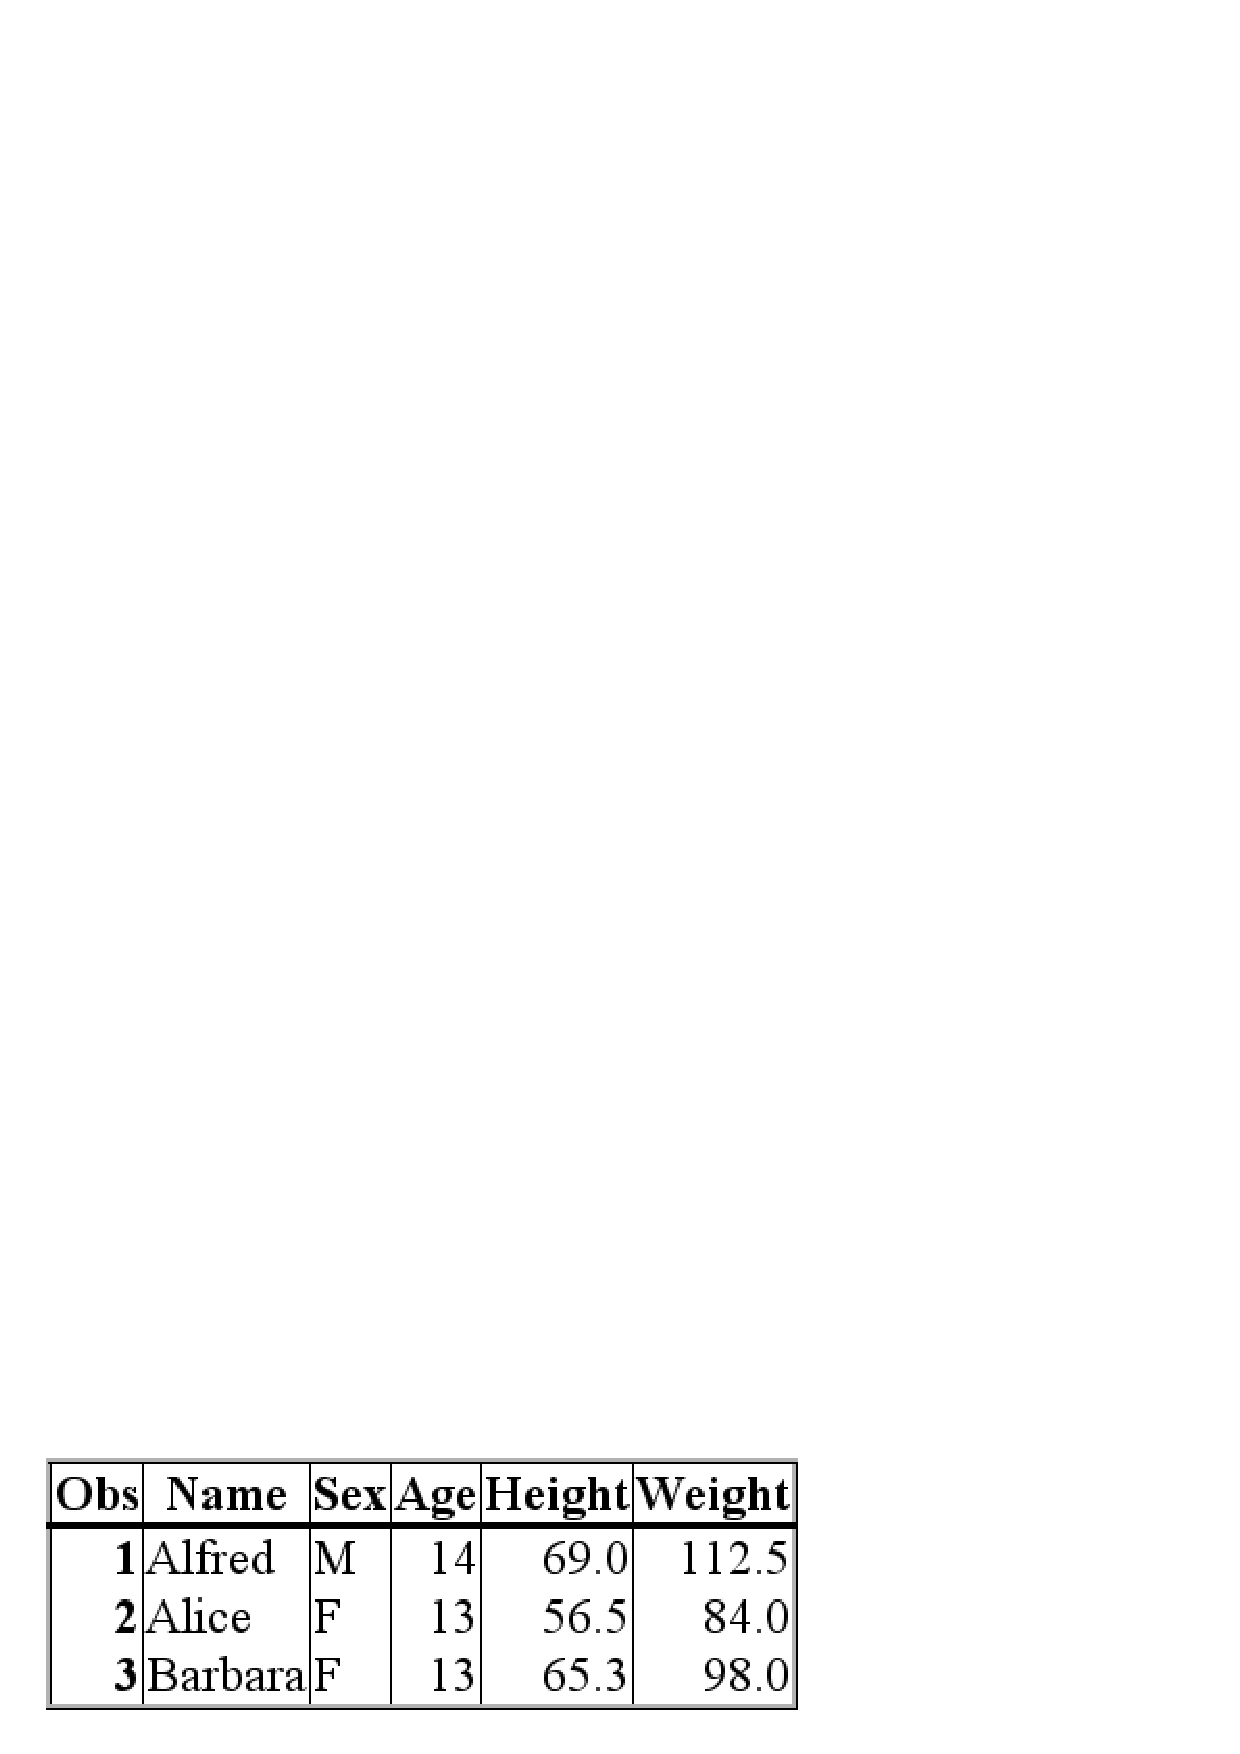
\includegraphics[width=6in]{table_rules1.png}
\end{goutput}

\subsection{Table Rules with style}
\index{Events!table\_head}
\index{Styles!table\_head}
Hard coding the style information in the tagset event is certainly
an easy solution.  But there is a better solution.  By using styles
the tagset can be made that will adapt to any need.  All that is really
needed is a style for the table\_head.  Then the tagset needs to use
that style.

Create a new style element for the table\_head is easy.  Setting 
the style on the table\_head
event is also easy.  The only thing that may not be so obvious is that
it is no longer necessary to put a style attribute on the thead tag.
All that is needed is a class attribute that will reference the new
style element.

\subsection{The Better Solution}
The new style and tagset is shown
in figure \ref{table_rules2} on page \pageref{table_rules2}.
The output from this job looks identical to the previous output. The
only difference is the implementation.

\begin{fvcode}{table_rules2}{Table rules with style}

proc template;

    define style styles.table_rules;

        style table /
          borderwidth=3
          bordercolor=black
          rules=cols
        ;

        style table_head /
          borderbottomstyle=solid
        ;
     end;

    define tagset tagsets.table_rules;
        parent=tagsets.html4;

        define event table_head;
            style=table_head;
            start:
                put '<thead'
                putq 'htmlclass=' htmlclass;
                put '>' nl;
            finish:
                put '</thead>' nl;
        end;
    end;
run;

ods tagsets.table_rules file='table.html' style=table_rules;
options obs=3;
proc print data=sashelp.class; run;
ods _all_ close;
\end{fvcode}

This is now a very flexible tagset that will work for anyone.
If no table\_head style is defined then it will behave as always.
But if it is defined, the table head will do whatever is asked 
of it.  

Excercise: Expand on this idea by applying it to the table\_body
and table\_foot events.  Play with the style attributes to see what happens.

\section{Everyone likes stripes}
\index{Table!Striped}
\index{Styles!data}
\index{Styles!dataStrong}
\index{Styles!dataEmphasis}
Another common request is to create tables with striped rows.  This is another
thing that is quite easy to do with styles.  A new style is needed to contrast the
data style already in use.  Then each row should switch between the data style and
the new style.  This is especially easy in SAS 9.1 because of do blocks.

It should be noted, that this can also be done with table templates.  However, 
table templates do not apply to the Report, Tabulate or Print procedures.

\subsection{Defining the Problem}
The goal for this solution is to stripe the data but not the headers or footers.
Reusing existing style elements would be ideal. But creating a new style is not 
out of the question.

\index{Styles!dataStrong}
\index{Styles!dataEmphasis}
\index{Variables!Section}
This is all easy enough to do.  There is a tagset variable called section that
indicates which part of the table the current row is in.  The possible values are head, body,
and foot.  There are also other data style elements available.  Most if not all
styles define dataStrong and dataEmphasis style elements in addition to the data
style.  One of those could be alternated with the data style.  Looking at some of
the style definitions shows that some of them only make the text bold or italic
for these style elements.  That may be too subtle.

For flexibility it would be nice to specify the alternate row style on the ods
statement.  If none is given then the tagset can assume it should use the dataStrong
style.


\subsection{The HTML solution}
\index{Events!classAlign}
\index{HTML!Justification}
\index{HTML!Class}
\index{Tagsets!html4}
\index{Tagsets!htmlcss}
There is no real need to identify and locate these events.  The data, header, row,
and table events figure prominently in most tagsets.
The only real complexity comes when examining the row and data events
in the html4 and htmlcss tagsets.  Instead of just 
printing the htmlclass it triggers an event called classAlign.  This is because
the html output creates a class attribute that has two class names.  One is
for the style and the other is for justification.  Now the classAlign event
needs to be redifined as well. If possible it is best to
preserve the current behavior of any modified events.  In this case the
behavior can be preserved by conditionally limiting the modification to 
only occur when the htmlcass is set to 'data'.

\subsection{The Code}
The finished html tagset is shown below. The striped tabular output is shown 
in figure \ref{striped_table_out} on page \pageref{striped_table_out}.

\begin{fvcode}{striped_table}{The striped table tagset}

proc template;

    define style styles.stripes;
        parent=styles.default;
    
        style DataStripe from data /
            background=cxE0E0E0
        ;
        
    end;
    
    define tagset tagsets.stripes;
        parent=tagsets.html4;

        define event initialize;

            do /if $options;
                 
                set $alt_row_style $options['ROW_STYLE'];
            done;

            set $alt_row_style 'datastrong' /if !$alt_row_style;
        end;

        define event options_set;
            trigger initialize;
        end;

        define event table_head;
            style=table_head;
            start:
                put '<thead';
                putq 'htmlclass=' htmlclass;
                put '>' nl;
                set $row_class 'data';
            finish:
                put '</thead>' nl;
        end;

        define event row;
            start:
                put '<tr>' nl;

            finish:
                put '</tr>' nl;

                do /if cmp(section, 'body');
                    do /if cmp($row_class, 'data');
                        set $row_class $alt_row_style;
                    else;
                        set $row_class 'data';
                    done;
                done;
        end;

        define event classalign;
            do /if cmp(htmlclass, 'data');
                set $class $row_class;
            else;
                set $class htmlclass;
            done;

            unset $vjust;
            unset $just;
            set $vjust vjust / when !cmp("t", vjust);
            set $just just / when !cmp("l", just);
            set $just "r" /when cmp("d", $just);
            break / when !any($class, $just, $vjust);
            put ' class="';
            put $just ' ' $vjust;
            put ' ' $class;
            put '"';
        end;
    end;
run;

ods tagsets.stripes file='striped.html' 
                   options(row_style='datastripe') 
                   style=stripes;
options obs=5;
proc print data=sashelp.class; run;
ods _all_ close;
\end{fvcode}

\begin{goutput}{striped_table_out}{Striped Tables}
\includegraphics[width=6in]{striped.png}
\end{goutput}

\subsection{The LaTeX solution}
\index{Table!Striped}
\index{LaTeX}
\index{Events!Header}
Doing this same example in LaTeX is even easier.  Mostly because
the LaTeX tagset is not as complicated as the html tagset.
The only difficulty comes from the header event.  The header event
in latex looks like this.
\begin{sfvcode}
        define event header;
            start:
               trigger data;
            finish:
               trigger data;
        end;
\end{sfvcode}

\index{Else}
\index{Statements!Else}
This is fine until the stylename that get's printed is the row\_class
variable.  The result is that all of the header cells are
missing their header references.  The fix was to do this in the data
event.   A Do / else block would be more efficient, but this works
just fine too.
\begin{sfvcode}
        put $row_class /if !cmp(event_name, 'header');
        put htmlclass  /if cmp(event_name, 'header');
\end{sfvcode}

\subsection{The Code}
The finish tagset is shown below. The output is shown 
in figure \vref{striped_table2_out}.

\begin{fvcode}{striped_table2}{Striped tables complete}

proc template;

    define tagset tagsets.striped_latex;
        parent=tagsets.colorlatex;

        define event initialize;

            do /if $options;
                 
                set $alt_row_style $options['ROW_STYLE'];
            done;

            set $alt_row_style 'datastrong' /if !$alt_row_style;
        end;

        define event options_set;
            trigger initialize;
        end;

        define event table_body;
            start:
                set $row_class 'Data';
            finish:
                unset $row_class;
        end;

        define event row;
            finish:
                put CR '\\\hline' CR;

                do /if cmp(section, 'body');
                    do /if cmp($row_class, 'Data');
                        set $row_class $alt_row_style;
                    else;
                        set $row_class 'Data';
                    done;
                done;
        end;

        define event data;
            start:
                put VALUE /if cmp($sascaption, 'true');
                break /if cmp($sascaption, 'true');
                put ' & ' CR / if !cmp(COLSTART, '1') ;

                /* Print cell formatting including class name and alignment. */
                put '   ';
                put '\multicolumn{';
                put colspan;
                put '1' / if !exists(colspan);
                put '}';
                put '{|S{';
                put $row_class /if !cmp(event_name, 'header');
                put htmlclass  /if cmp(event_name, 'header');
                put '}{';
                put just;
                put '}|}';
                put '{';
                put VALUE;

            finish:
                break /if cmp($sascaption, 'true');
                put '}';
        end;
 
    end;
run;

ods tagsets.striped_latex 
    file='striped.tex' 
    style=stripes 
    options(row_style="DataStripe");

options obs=5;
proc print data=sashelp.class; run;
ods _all_ close;
\end{fvcode}


\begin{table}\caption{Striped LaTeX Table}
\label{striped_table2_out}
\begin{sastable}[c]{rllrrr}\hline
   \multicolumn{1}{|S{Header}{c}|}{Obs} & 
   \multicolumn{1}{|S{Header}{c}|}{Name} & 
   \multicolumn{1}{|S{Header}{c}|}{Sex} & 
   \multicolumn{1}{|S{Header}{c}|}{Age} & 
   \multicolumn{1}{|S{Header}{c}|}{Height} & 
   \multicolumn{1}{|S{Header}{c}|}{Weight}
\\\hline
   \multicolumn{1}{|S{RowHeader}{r}|}{ 1} & 
   \multicolumn{1}{|S{Data}{l}|}{Alfred} & 
   \multicolumn{1}{|S{Data}{l}|}{M} & 
   \multicolumn{1}{|S{Data}{r}|}{14} & 
   \multicolumn{1}{|S{Data}{r}|}{69.0} & 
   \multicolumn{1}{|S{Data}{r}|}{112.5}
\\\hline
   \multicolumn{1}{|S{RowHeader}{r}|}{ 2} & 
   \multicolumn{1}{|S{DataStripe}{l}|}{Alice} & 
   \multicolumn{1}{|S{DataStripe}{l}|}{F} & 
   \multicolumn{1}{|S{DataStripe}{r}|}{13} & 
   \multicolumn{1}{|S{DataStripe}{r}|}{56.5} & 
   \multicolumn{1}{|S{DataStripe}{r}|}{ 84.0}
\\\hline
   \multicolumn{1}{|S{RowHeader}{r}|}{ 3} & 
   \multicolumn{1}{|S{Data}{l}|}{Barbara} & 
   \multicolumn{1}{|S{Data}{l}|}{F} & 
   \multicolumn{1}{|S{Data}{r}|}{13} & 
   \multicolumn{1}{|S{Data}{r}|}{65.3} & 
   \multicolumn{1}{|S{Data}{r}|}{ 98.0}
\\\hline
   \multicolumn{1}{|S{RowHeader}{r}|}{ 4} & 
   \multicolumn{1}{|S{DataStripe}{l}|}{Carol} & 
   \multicolumn{1}{|S{DataStripe}{l}|}{F} & 
   \multicolumn{1}{|S{DataStripe}{r}|}{14} & 
   \multicolumn{1}{|S{DataStripe}{r}|}{62.8} & 
   \multicolumn{1}{|S{DataStripe}{r}|}{102.5}
\\\hline
   \multicolumn{1}{|S{RowHeader}{r}|}{ 5} & 
   \multicolumn{1}{|S{Data}{l}|}{Henry} & 
   \multicolumn{1}{|S{Data}{l}|}{M} & 
   \multicolumn{1}{|S{Data}{r}|}{14} & 
   \multicolumn{1}{|S{Data}{r}|}{63.5} & 
   \multicolumn{1}{|S{Data}{r}|}{102.5}
\\\hline
\end{sastable}
\end{table}

\subsection{Summary}
With just a little extra effort the striped tagsets provide enough
flexibility to be useful with any style.  They can even provide
different looks by using different style elements within the chosen
style.  If the style doesn't provide a suitable style element then
it is still easy to inherit from that style and add a single element
to do the striping.

Excercise:  It would be a worthwhile to play with different
styles and style elements to see what sort of striping you might
get.

\section{slidebar columns}
This is a great example of what can be done with a little
imagination.  This example takes advantage of cell widths
as percentages, to create a bar chart affect within a table column.

\subsection{Define the Problem}
The desire is to use a numeric or percentage value and 
create a sliding bar that reflects the value.  If it's a percentage
everything is very easy.  If it is a numeric value then things get
a little more complicated.  Those cases will need some sort of maximum
value to create a percentage from.  Another need is how to
identify the column to use.  For this, styles will be used in a new way.

The HTML implementation of the slidebar is done by creating a table 
inside the data cell.  The table will have 2 cells inside of it.  
The first one will use a percentage width to create a bar.  A little bit of
HTML editing shows that a table cell like this one will give the
desired effect.

\begin{sfvcode}
    <td width="150">
      <table width="100%">
        <td width="72%">72</td><td>&nbsp;</td>
      </table>
    </td>
\end{sfvcode}

\index{Style!Attributes!TagAttr}
\index{Style!Attributes!HTMLClass}
\label{slider}
There is a style attribute called TagAttr.  It stands for Tag Attribute.
TagAttr was meant as a catch all
for any new browser features that styles did not directly accomodate.
Normally anything in TagAttr is printed as is within the tag it belongs
to.  This tagset is going to misuse TagAttr so that proc print can say which columns
should get a slide bar.  It can also be used to give the maximum value for
columns that are not percentages.

\subsection{Identify and Locate}
This step get's easier as tagset events become familiar.  
In this case everything revolves around the data event. 

\subsection{The Solution}
Let's get on with the code. 

\begin{fvcode}{final_slider}{Slider Tagset Complete}
proc template;
    define style styles.slider;
        parent=styles.default;

        style table from output /
            rules=cols
            cellpadding=3
            cellspacing=1
        ;
        style slider from data /
            background=colors('headerbg')
        ;
    end;
  
    define tagset tagsets.slider;
        parent=tagsets.html4;

        define event calculate_width;
            set $width value /breakif index(value, '%') > 0;

            eval $dash_pos index(Tagattr, '-');
            do /if $dash_pos;
                eval $dash_pos $dash_pos+1;
            done;
            eval $value inputn(value, '12.');
            eval $max inputn(substr(Tagattr, $dash_pos), '12.');
            eval $width ($value / $max) * 100;
            set $width $width '%';
            unset $dash_pos;
        end;

        define event data;
            start:
                /* this would work but sometimes htmlclass is empty... */
                trigger header /breakif cmp(htmlclass, "RowHeader");
                trigger header /breakif cmp(htmlclass, "Header");

                do /if index(tagattr, 'slider') > 0;
                    put '<td width="150" class="data">' nl;
                    put '<table width="100%" class="data" cellpadding=0; cellspacing=0;>' nl;
                    trigger calculate_width;
                done;
                put "<td";
                putq ' width=' $width;
                putq " title=" flyover;
                do /if !cmp(htmlclass,'batch');
                    trigger classalign;
                    trigger style_inline;
                done;
                trigger rowcol;
                put " nowrap" /if no_wrap;
                put ">";
                trigger cell_value;

            finish:
                trigger header /breakif cmp(htmlclass, "RowHeader");
                trigger header /breakif cmp(htmlclass, "Header");
   
                trigger cell_value;
                put "</td>" CR;
                do /if $width;
                    put '<td>&nbsp;</td>' CR;
                    put "</table></td>" CR;
                    unset $width;
                done;

        end;
    end;
run;

options obs=3;
ods tagsets.slider file='test.html' style=slider;

proc print data=sashelp.class;
    var name;
    var sex;
    var age;     
    var height / style(data) = slider[just=center tagattr="slider-80"];
    var weight / style(data) = slider[just=center tagattr="slider-150"];
run;

ods tagsets.slider close;
\end{fvcode}        

The output from this example can be seen in figure \vref{slider_out}.
The heart of this example is the data event.  
All it needed was an if block that would create a table with two
cells inside what would ordinarily be a simple data cell.  The first cell
in the slider table is created with the code that normally creates the data
cell.  It just adds the \$width variable if it is there.  The finish
of the data event adds the extra empty cell and closes everything up.

The most complicated part of the tagset is the calculate\_width event.
This is mostly because sliders will work for numeric values as well as
percentages.
If the tagset only worked with pecentages this event wouldn't have been needed.

There is also a short style to make the table look a little nicer.  
Using less cellspacing and padding along with column rules looks nice.  
This example could be combined with the first example in this chapter
for an even nicer look.

The last piece of the puzzle is using the print Procedure's style over-ride
capabilities to turn the sliders on and give a max value to calculate
the percentages from.  A macro variable could have been used to
indicate which columns to use, but this is a little bit nicer.

Excercise:  Create a slider tagset that uses a macro variable or style
over-ride to create sliders on the the columns indicated.

\begin{goutput}{Slider_out}{Slider Columns}
\includegraphics[width=6in]{slider.png}
\end{goutput}

\subsection{Example Summary}
In this example the tagattr style attribute was used to indicate the 
slider columns and the
maximum value.  But since a slider style element was also created the
tagset could just as easily key off of the value of htmlclass and only 
use tagattr to indicate a maximum value if needed.

Exercise: Find and eliminate the extra printing of Tagattr in the data tags.

Exercise: Change the tagset to key off of the style element name instead of
the keyword 'slider' in tagattr.

Exercise: Change the inheritance of this tagset to take advantage of the
changes made to the table\_rules tagset in figure \ref{table_rules2} on page
\pageref{table_rules2}. Combine the table\_rules style with
the slider style.

Exercise: Combine all the examples in the chapter into one tagset.

\section{Summary}
This chapter has shown how styles can be used with tagsets to easily create
nice output.  Using styles can simplify solutions and make those solutions
more adaptable. 

%%\cleardoublepage
%%\include{chapter9}
%%\cleardoublepage
%%\include{chapter10}
%%\cleardoublepage
%%\chapter{Datastep Conversions}
\index{DataStep Conversions}
You may wonder, why would someone want to convert a datastep 
program to use tagsets?  There are lots of reasons.  Mostly it's
for code reuse and flexibility.  Datastep programs allow lots of
flexibility but they are written for one purpose.  If the same 
functionality is desired for a different set of data an entirely
new datastep will have to be written.  If the rendering is left to
a tagset, then anyone can use that tagset with any form of data,
and any procedure.  Maintenance of the code is also simplified 
since both the tagset and the resulting SAS job wil be much
simpler than the original datastep. Add the various powers of
ODS to this new found flexibility and there is plenty of motivation
for conversion.  This chapter will show the process and rewards 
of converting datastep programs to tagsets. 

\index{DDE}
\index{CSV}
\index{XML}
Yet another reason to
convert is that tagsets can be interchanged to create new and 
diffrent outputs.  Usually datastep is used to create HTML, CSV,
or DDE to XML,  A different datastep is required for each.  A different
tagset is required for each as well.  The difference is the reusability
and the ease of creation and maintenance.

\index{ODS}
\index{ODS!Styles}
\index{ODS!Select}
\index{ODS!Exclude}
\index{ODS!Document}
Full integration with ODS provides more than enough reasons to convert 
a datastep to a tagset.  Ods styles, table templates, select and exclude,
and proc document are very good reasons.  There are many other things that
ODS can do besides these, but not if datastep is the method of creating the
output.

\section{Special Bylines}
\index{nobs}
\index{Counting Observations}
\index{Bylines}
One of the things that can be done in datastep is the counting of observations
for display in the byline.  The datastep just counts them first then another
datastep prints everything out.  Tagsets can do that too.  This first example
has a special style, as well as a special byline.  The byline text may change
based upon the current by value.  Each byline also displays the number of
observations in the table below it.  

\subsection{The DataStep Code}
\index{Procedures!Report}
\index{Highlighting}
The original datastep code is shown below.  It has been simplified to use
the sashelp.class dataset.  There is nothing very hard about this code.  The
worst thing is all the puts.  The original data step also did some highlighting
and value translation.  Both of those things are much easier to do using the report procedure.
Another nice thing this datastep does is put the web page title in the title tag and
as the heading on the page.  This is also easy to do with a tagset. The original
output can be seen in figure \vref{ages_out}.

\begin{sfvcode}
filename webout 'ages.html';

%let numfuture=16;

proc sort data=sashelp.class out=myclasssrt;
  by age name weight;
run;

/* Count number of items in each BY group */
data cnt_by_obs;
   keep cnt;

   set work.myclasssrt;
   by age;

   if first.age then curcnt = 0;
   curcnt + 1;
   if last.age then do; cnt = curcnt; output; end;
run;

options missing='-';
data _null_;
   file webout;
   if _N_ = 1 then do;
      length title $ 128;
      length stoday stime $ 8;
      retain linecnt 1;

      stoday = put( today(), date7. );
      stime = put( time(), time5. ); 
      title = 'Class List &nbsp;-&nbsp; ' || stoday || "at " || stime;
      put '<!DOCTYPE HTML PUBLIC "-//IETF//DTD HTML//EN">';
      put '<HTML><HEAD>';
      put '<TITLE>' title '</TITLE>';
      put '</HEAD><BODY>';
      put '<CENTER><H3>' title '</H3></CENTER>';
   end;

   set work.myclasssrt;
   by age;

   if _N_ = 1 or FIRST.age then do;
      length lab $ 32;
      set work.cnt_by_obs;
      if age >= &numfuture then do;
         put '<CENTER><B><FONT SIZE=+2>The Oldest</FONT> ' @;
         put '<FONT SIZE=-1>(' cnt +(-1) ' '@;
         if cnt = 1 then
            put 'entry)' @;
         else
            put 'entries)' @;
         put '</FONT></B></CENTER>';
      end;
      else do;
         put '<CENTER><B><FONT SIZE=+2>Age is ' age '</FONT> ' @;
         put '<FONT SIZE=-1>(' cnt +(-1) ' '@;
         if cnt = 1 then
            put 'entry)' @;
         else
            put 'entries)' @;
         put '</FONT></B></CENTER>';
      end;
      put '<TABLE ALIGN=CENTER VALIGN=MIDDLE>';
      put '<TR>';
      lab = vlabel(Name);         put '<TH>' lab '</TH>';
      lab = vlabel(Weight);       put '<TH>' lab '</TH>';
      lab = vlabel(Height);       put '<TH>' lab '</TH>';
      lab = vlabel(Sex);          put '<TH>' lab '</TH>';
      put '</TR>';
   end;

   if mod(linecnt,2) then
      put '<TR ALIGN=CENTER VALIGN=MIDDLE BGCOLOR="D5E5D2">';
   else
      put '<TR ALIGN=CENTER VALIGN=MIDDLE>';

   put '<TD ALIGN=CENTER>' name '</TD>';
   put '<TD><FONT SIZE=-1>' weight '</FONT></TD>';
   put '<TD><FONT SIZE=-1>' height '</FONT></TD>';
   put '<TD><FONT SIZE=-1>' sex '</FONT></TD>';
   put '</TR>';

   linecnt + 1;

   if LAST.age then do;
      put '</TABLE>';
      linecnt = 1;
      put '<BR><HR><BR>';
      put '</BODY></HTML>';
   end;
run;

\end{sfvcode}

\begin{goutput}{ages_out}{Data step}
\includegraphics[width=4in]{ages.png}
\end{goutput}


\subsection{Breaking it down}
\index{Styles!Minimal}
The best way to approach a problem like this is to break it down into separate
problems.  In this case there is a fairly minimalist set of colors and fonts.
A fairly simple ODS style can be created from what can be seen in the datastep code.

\index{Tables!striping}
The next problem is striping of tables.  That problem was solved in the example on
page \pageref{striped_table}.
So this new tagset can use the stripes tagset as it's parent.  

\index{Byline!Modifying}
\index{Counting Observations}
There are three more things to solve, Extending the use of the title, counting the 
observations, and modifying the byline.  It would be perfectly
reasonable to solve both those problems in one tagset.  But the last
tagset is simpler if an
intermediate tagset is created to count the observations and display the count.
As a bonus the intermediate tagset can be used in other jobs to solve
other problems because it is not specific to this specific problem.

\subsection{The Style}
\index{Styles!Minimal}
Extracting all the colors and fonts from the datastep is easy enough.  
With something this simple the best thing is to use the minimal style as
a parent.  The minimal style will provide everything that is needed 
without making things complicated.
The resulting style looks like this.

\begin{sfvcode}
    define Style styles.minimal_striped; 
        parent = styles.minimal;

        style header/
            font = (, 4,bold)
        ;

        style Data/
            font = (, 3,normal)
        ;

        style DataStrong from data /
            background=cxD5E5D2
        ;

        replace Output /
            BorderWidth = 0
            CellSpacing = 1
            CellPadding = 7
            Frame = void
            Rules = none
        ;

    end;
\end{sfvcode}


\subsection{Counting Observations}
\index{Observation Count}
\index{Number of Observations}
\index{nobs}
\index{Variables!Macro}
The new tagset inherits from tagsets.stripes from page \pageref{striped}. 
This tagset manipulates the title and prints it as a heading. 
We also add a counter for the observations, and a stream to catch
the table while the observations are being counted.  The last thing is to add
an event to print the observation count.
A macro variable called do\_nobs\_label must be set to 'true' for the observation
counting to take effect.  Otherwise the tagset will exhibit normal behavior.
This tagset will work for any tabular output that ods creates.  
The new tagset looks like this.  
The Output is shown in listing \vref{ages2_out}.

\begin{sfvcode}
proc template;
    define tagset tagsets.nobs_label;
        parent=tagsets.stripes;

        define event initialize;
            unset $do_nobs;
            do /if $options;

                set $do_nobs "true" /if cmp($options['NOBS_LABEL']), 'yes');

                /*---------------------------------------------------eric-*/
                /*-- From the stripes tagset.                           --*/
                /*------------------------------------------------9Nov 03-*/
                set $alt_row_style $options['ALTERNATE_STYLE']";
            done;

            set $alt_row_style 'DataStrong' /if !$alt_row_style;
        end;    

        define event options_set;
            trigger initialize;
        end;

        /*-------------------------------------------------------eric-*/
        /*-- Add the date and time to the document title.  Save it  --*/
        /*-- away for later.                                        --*/
        /*----------------------------------------------------7Aug 03-*/
        define event doc_title;
              break /if ^value;
              set $title value '&nbsp;-&nbsp;' date " at " time; 
              putl '<TITLE>' $title '</TITLE>';
        end;

        define event doc_body;
            start:
                put '<body onload="startup()"';
                put ' onunload="shutdown()"';
                put  ' bgproperties="fixed"' / WATERMARK;
                putq " class=" HTMLCLASS;
                putq " background=" BACKGROUNDIMAGE;
                trigger style_inline;
                put ">" nl;
                trigger pre_post;
                put          nl;
                trigger ie_check;

                /*-----------------------------------------------eric-*/
                /*-- This is the part that changed.                 --*/
                /*-- Add in the title if we have one.               --*/
                /*--------------------------------------------7Aug 03-*/
                do /if $title;
                    putl '<h3';
                    trigger align;
                    putl '>' $title '</h3>';
                done;

            finish:
                trigger pre_post;
                put "</body>" nl;
        end;

        define event output;
            finish:
                put "<br>" nl;
        end;

        define event table ;
            start:
                eval $nobs 0;
                
                /*-----------------------------------------------eric-*/
                /*-- if we are not going to print the nobs label   --*/
                /*-- then there is no point in doing extra work.   --*/
                /*--------------------------------------------7Aug 03-*/
                open table /if cmp($do_nobs, 'true');
                set $row_class 'data';
                
                put "<div";
                trigger alt_align;
                put ">" CR;
                put '<table>' nl;
            finish:
                put '</table>' nl;
                put "</div>" nl;
                
                /*-----------------------------------------------eric-*/
                /*-- if we are not going to print the nobs label   --*/
                /*-- then there is no point in doing extra work.   --*/
                /*--------------------------------------------7Aug 03-*/
                do /if cmp($do_nobs, 'true');
                    close;
                    /* print the nobs */
                    trigger table_nobs_label; 

                    /* print the table */
                    put $$table;
                    unset $$table;
                done;
        end;
        
        /*-------------------------------------------------------eric-*/
        /*-- Count the data rows.  Swap colors.                     --*/
        /*----------------------------------------------------7Aug 03-*/
        define event row;
            start:
                /*-----------------------------------------------eric-*/
                /*-- Don not count unless we are in the data.       --*/
                /*--------------------------------------------7Aug 03-*/
                putq '<tr>' nl;
                do /if cmp(section, 'body');
                    eval $nobs $nobs+1 ;
                done;
            finish:
                put '</tr>' nl;
                /*-----------------------------------------------eric-*/
                /*-- Swap the row style at the end of the row.      --*/
                /*-- That way the first row is the one we set in    --*/
                /*-- table start.                                   --*/
                /*--------------------------------------------7Aug 03-*/
                trigger swapclass /if cmp(section, 'body');
        end;
        

        /*-------------------------------------------------------eric-*/
        /*-- Print a small heading above the table.                 --*/
        /*-- (## entries)                                           --*/
        /*----------------------------------------------------7Aug 03-*/
        define event table_nobs_label;
            style=nobs_label;
            put '<p><h4';
            putq ' class=' htmlclass; 
            put ' style="text-align: center">(' $nobs ' ';
            do /if $nobs = 1; 
                put 'entry)' ;
            else;
                put 'entries)' ;
            done;
            put '</h4></p>';
        end;
        
    end;
run;

title;


ods tagsets.nobs_label options(nobs_label='yes') 
    file="ages2.html" (title='Class List')
    style=minimal_striped;

proc sort data=sashelp.class out=myclasssrt;
    by age name sex height weight;
run;

proc print data=work.myclasssrt noobs;
    by age;
    pageby age;
run;

ods tagsets.table_nobs close;
\end{sfvcode}

\begin{goutput}{ages2_out}{Observation Counts}
\includegraphics[width=5in]{ages2.png}
\end{goutput}

\subsection{various problems}
\index{Events!table\_head}
\index{Style!table\_head}
The first time this job runs, there is a warning in the log that the table\_head style
was not found.  This is coming from the stripes tagset where the table\_head event
is asking for the table\_head style.  It doesn't really cause any problems but defining
an empty style will take care of the warning.

\begin{sfvcode}
   style table_head
   ;
\end{sfvcode}
 
The other thing that is needed is a style for the number of observations label.  The style has
now grown to look like this.

\begin{fvcode}{datastep_style}{Refined striped style}
    define Style styles.minimal_striped; 
        parent = styles.minimal;

        style header/
            font = (, 4,bold)
        ;

        style Data/
            font = (, 3,normal)
        ;

        style DataStrong from data /
            background=cxD5E5D2
        ;

        style nobs_label from data /
        ;

        style table_head
        ;

        style byline /
           font_size = 5
           font_weight = bold
        ;

        replace Output /
            BorderWidth = 0
            CellSpacing = 1
            CellPadding = 7
            Frame = void
            Rules = none
        ;

    end;
\end{fvcode}


\subsection{Modifying the Byline}
\index{Byline!modification}
All that is left is for the byline to modified to match what the datastep code did.
This part isn't too hard either.  The easiest way to do this is to code it for the
data we are reporting on.  That makes this tagset specific to the task, and not
very reusable.  But it is a good first step.

\index{Variables!Macro}
\index{Events!Nobs\_label}
\index{Events!Byline}
Another option will work nicely to indicate which byline needs to be modified. Luckily
only one by value needs changing.  The end of the byline can be postponed until the 
table ends.  That means that the nobs event from the nobs\_count tagset can handle most 
of the work.  In the interest of versatility the byline and nobs\_label events have
been set up to work together.  If there is no byline, the nobs\_label event handles
the situation by doing the setup that the byline event would have done if there was a byline.

The new tagset and it's output follows.

\begin{fvcode}{by_age_tagset}{Tagset with modified by lines}
    define tagset tagsets.by_age;
        parent=tagsets.nobs_label;
        
        /*-------------------------------------------------------eric-*/
        /*-- Add some extra comments to the doc event.              --*/
        /*----------------------------------------------------8Aug 03-*/
        define event initialize;
            unset $do_nobs;
            do /if $options;

                do /if $options['MODIFY_BY'];
                    eval $modify_by inputn($options['MODIFY_BY'], '7.');
                    do /if missing($modify_by);
                        eval $modify_by 0;
                    done;
                done;

                set $do_nobs "true" /if cmp($options['NOBS_LABEL']), 'yes');

                /*---------------------------------------------------eric-*/
                /*-- From the stripes tagset.                           --*/
                /*------------------------------------------------9Nov 03-*/
                set $alt_row_style $options['ALTERNATE_STYLE']";
            done;

            set $alt_row_style 'DataStrong' /if !$alt_row_style;

        end;    


        /*-------------------------------------------------------eric-*/
        /*-- We want to say two different things depending on the   --*/
        /*-- value in the byline.                                   --*/
        /*----------------------------------------------------7Aug 03-*/
        define event byline;
            /*---------------------------------------------------eric-*/
            /*-- Convert age to a numeric.                          --*/
            /*------------------------------------------------7Aug 03-*/
            eval $byval inputn(scan(value, -1, '='), '7.');
        
            put '<p><div';
            putq ' class=' htmlclass ;
            put ' style="text-align: center;">' nl;

            do /if $byval = $modify_by ;
                put 'The Oldest';
            else;
                put 'Age is ' $byval ;
            done;
            
            /*---------------------------------------------------eric-*/
            /*-- A newline would do, but one way or another we need --*/
            /*-- to flush.  Otherwise the timing goes sour.         --*/
            /*------------------------------------------------8Aug 03-*/
            flush;
            set $byline "true";
        end;
        

        /*-------------------------------------------------------eric-*/
        /*-- The nobs title finishes up the paragraph started with  --*/
        /*-- the byline.                                            --*/
        /*----------------------------------------------------7Aug 03-*/
        define event table_nobs_label;
            style=nobs_label;

            /*---------------------------------------------------eric-*/
            /*-- If we did not get a byline then we want to make    --*/
            /*-- sure the html is still well formed.                --*/
            /*------------------------------------------------8Aug 03-*/
            do /if ^$byline;
                put '<p><div';
                putq ' class="byline"';
                put ' style="text-align: center">' nl;
                unset $byline;
            done;

            put '&nbsp;&nbsp;<span class="' htmlclass '">(' $nobs ' ';

            do /if $nobs = 1; 
                put 'entry)' ;
            else;
                put 'entries)' ;
            done;

            put '</span></div></p>' nl;
        end;

    end;
\end{fvcode}

The proc print that creates this output is still rather simple.  Only the two
macro variables look out of the ordinary.

\begin{sfvcode}
title;

ods tagsets.by_age options(nobs_label='yes' modify_by='16')
    file="ages3.html" (title='Class List')
    style=minimal_striped;

proc sort data=sashelp.class out=myclasssrt;
  by age name sex height weight;
run;

*options obs=6;

proc print data=work.myclasssrt noobs;
    by age;
    pageby age;
run;

ods tagsets.by_age close;
\end{sfvcode}


\begin{goutput}{ages3_out}{Output with modified By lines}
\includegraphics[width=4in]{ages3.png}
\end{goutput}

\subsection{A more flexible solution}
\index{Events!Byline}
\index{Dictionary}
This tagset is simple enough that it doesn't really matter that it's specific to this
data.  But with a little work it can be made more universal.  All it needs is a more
flexible way to indicate which by values need reformatting, and what they should be 
reformatted to.  That can be done with a macro variable. The heart of this tagset
is a dictionary.  When the proc starts the macro variable is parsed and put in 
the dictionary.  The byline event uses the dictionary to decide what to do with
each byline.  

\index{Events!Bygroup}
\subsubsection{More Identify, and Locate}
\index{ByLines}
There is an event called bygroup that surrounds all bygroup processing.  Using the start
of that event to parse the macro variable and set up the by value dictionary for the by lines
that will be coming. All of this requires that the by values are known.  But that
was a prerequesite for this particular problem anyway.

The new mod\_by\_line tagset follows.

\begin{fvcode}{flexible_byline_tagset}{A more versatile byline tagset}
 define tagset tagsets.mod_by_line;
        parent=tagsets.nobs_label;
        
        define event bygroup;
            start:
                /*-----------------------------------------------eric-*/
                /*-- Do not do this if there is no need.            --*/
                /*--------------------------------------------9Nov 03-*/
                break /if ^modify_by;

                break /if cmp($modify_by, modify_by);
                
                unset $byval_subs;
                set $modify_by modify_by;
                
                eval $count 1;
                trigger set_byval_pair;

                do /while !cmp($byval_pair, ' ');

                    set $byval_subs[$byval] $substitution;

                    eval $count $count+1;

                    trigger set_byval_pair;
                done;

        end;

        define event set_byval_pair;     
            set $byval_pair scan($modify_by, $count, '|');
            set $byval scan($byval_pair, 1, ':');
            set $substitution scan($byval_pair, 2, ':');
        end;   
        

        define event byline;
            /*---------------------------------------------------eric-*/
            /*-- Get the by value in string form                    --*/
            /*------------------------------------------------7Aug 03-*/
            eval $byval trim(scan(value, -1, '='));
            
            put '<p><div';
            putq ' class=' htmlclass ;
            put ' style="text-align: center;">' nl;

            do /if $byval_subs[$byval];
                put $byval_subs[$byval];
            else;
                do /if by_label;
                    put by_label $byval;
                else;
                    put value;
                done;
            done;
            
            /*---------------------------------------------------eric-*/
            /*-- A newline would do, but one way or another we need --*/
            /*-- to flush.  Otherwise the timing goes sour.         --*/
            /*------------------------------------------------8Aug 03-*/
            flush;
            set $byline "true";
        end;
        

        define event table_nobs_label;
            style=nobs_label;

            /*---------------------------------------------------eric-*/
            /*-- If we did not get a byline then we want to make    --*/
            /*-- sure the html is still well formed.                --*/
            /*------------------------------------------------8Aug 03-*/
            do /if ^$byline;
                put '<p><div';
                putq ' class=' htmlclass;
                put ' style="text-align: center">' nl;
                unset $byline;
            done;

            put '&nbsp;&nbsp;<span class="' htmlclass '">(' $nobs ' ';

            do /if $nobs = 1; 
                put 'entry)' ;
            else;
                put 'entries)' ;
            done;

            put '</span></div></p>' nl;
        end;

    end;
\end{fvcode}

\index{Debugging}
\index{Putlog}
\index{Statements!Putlog}
\index{Putvars}
\index{Statements!Putvars}
Tagsets like this are not all that difficult except that a mis-spelled variable or
an incorrect if statement will cause it to quietly not do what you asked.  A well placed
putlog or putvars statement can be very revealing.  In this case checking for
the options and memory variables looks like this.

\begin{sfvcode}
   putvars $options _name_ ':' _value_ ':' nl;
   putvars mem _name_ ':' _value_ ':' nl;
   putvars $byval_subs _name_ ':' _value_ ':' nl;
\end{sfvcode}

There are two things in these examples that help with debugging.  The placement
of a character on both sides of a value to reveal whitespace.  The other trick
is to separate the highly visible label from the variable by inserting another
string between them.  Then if the variable does not exist, the label will still
print.

\index{Variables!Macro}
The new job which uses the new macro variables is shown in the following job 
which creates the output in figure \ref{ages4_out} on page \pageref{ages4_out}.

\begin{sfvcode}
title;

ods tagsets.mod_by_line 
    options(nobs_label='yes' 
            by_label='Age is' 
            modify_by='16:The Oldest|11:The Youngest')
    file="ages4.html" (title='Class List')
    style=minimal_striped;

proc sort data=sashelp.class out=myclasssrt;
  by age name sex height weight;
run;

proc print data=work.myclasssrt noobs;
    by age;
    pageby age;
run;

ods tagsets.mod_by_line close;
\end{sfvcode}

\begin{goutput}{ages4_out}{Modifying Bylines, Final output}
\includegraphics[width=4in]{ages4.png}
\end{goutput}


\section{Summary}
This chapter has shown some of the advantages of converting datastep code
to tagsets.  Tagsets do not pretend to replace datastep, but if responsiblities
are divided between datastep and tagsets then the solution is more open for 
re-use in later solutions.  More power and flexibility is also provided by the
tight integration the output now has with ODS.


%%\cleardoublepage

%\part{Advanced Examples}
%{
%These chapters will cover more advanced examples.  These examples are
%more advanced because they do more than one thing at a time.  Multiple
%concepts are needed to accomplish these solutions.  These chapters will
%cover website integration, Data Step Conversions, repeating headers, 
%automatic paneling of output, and an extension of the slidebar example shown earlier.
%Understanding these examples is a good indication that all problems are within
%your grasp. 
%}

%%\include{chapter10}
%%\cleardoublepage
%%\chapter{Datastep Conversions}
\index{DataStep Conversions}
You may wonder, why would someone want to convert a datastep 
program to use tagsets?  There are lots of reasons.  Mostly it's
for code reuse and flexibility.  Datastep programs allow lots of
flexibility but they are written for one purpose.  If the same 
functionality is desired for a different set of data an entirely
new datastep will have to be written.  If the rendering is left to
a tagset, then anyone can use that tagset with any form of data,
and any procedure.  Maintenance of the code is also simplified 
since both the tagset and the resulting SAS job wil be much
simpler than the original datastep. Add the various powers of
ODS to this new found flexibility and there is plenty of motivation
for conversion.  This chapter will show the process and rewards 
of converting datastep programs to tagsets. 

\index{DDE}
\index{CSV}
\index{XML}
Yet another reason to
convert is that tagsets can be interchanged to create new and 
diffrent outputs.  Usually datastep is used to create HTML, CSV,
or DDE to XML,  A different datastep is required for each.  A different
tagset is required for each as well.  The difference is the reusability
and the ease of creation and maintenance.

\index{ODS}
\index{ODS!Styles}
\index{ODS!Select}
\index{ODS!Exclude}
\index{ODS!Document}
Full integration with ODS provides more than enough reasons to convert 
a datastep to a tagset.  Ods styles, table templates, select and exclude,
and proc document are very good reasons.  There are many other things that
ODS can do besides these, but not if datastep is the method of creating the
output.

\section{Special Bylines}
\index{nobs}
\index{Counting Observations}
\index{Bylines}
One of the things that can be done in datastep is the counting of observations
for display in the byline.  The datastep just counts them first then another
datastep prints everything out.  Tagsets can do that too.  This first example
has a special style, as well as a special byline.  The byline text may change
based upon the current by value.  Each byline also displays the number of
observations in the table below it.  

\subsection{The DataStep Code}
\index{Procedures!Report}
\index{Highlighting}
The original datastep code is shown below.  It has been simplified to use
the sashelp.class dataset.  There is nothing very hard about this code.  The
worst thing is all the puts.  The original data step also did some highlighting
and value translation.  Both of those things are much easier to do using the report procedure.
Another nice thing this datastep does is put the web page title in the title tag and
as the heading on the page.  This is also easy to do with a tagset. The original
output can be seen in figure \vref{ages_out}.

\begin{sfvcode}
filename webout 'ages.html';

%let numfuture=16;

proc sort data=sashelp.class out=myclasssrt;
  by age name weight;
run;

/* Count number of items in each BY group */
data cnt_by_obs;
   keep cnt;

   set work.myclasssrt;
   by age;

   if first.age then curcnt = 0;
   curcnt + 1;
   if last.age then do; cnt = curcnt; output; end;
run;

options missing='-';
data _null_;
   file webout;
   if _N_ = 1 then do;
      length title $ 128;
      length stoday stime $ 8;
      retain linecnt 1;

      stoday = put( today(), date7. );
      stime = put( time(), time5. ); 
      title = 'Class List &nbsp;-&nbsp; ' || stoday || "at " || stime;
      put '<!DOCTYPE HTML PUBLIC "-//IETF//DTD HTML//EN">';
      put '<HTML><HEAD>';
      put '<TITLE>' title '</TITLE>';
      put '</HEAD><BODY>';
      put '<CENTER><H3>' title '</H3></CENTER>';
   end;

   set work.myclasssrt;
   by age;

   if _N_ = 1 or FIRST.age then do;
      length lab $ 32;
      set work.cnt_by_obs;
      if age >= &numfuture then do;
         put '<CENTER><B><FONT SIZE=+2>The Oldest</FONT> ' @;
         put '<FONT SIZE=-1>(' cnt +(-1) ' '@;
         if cnt = 1 then
            put 'entry)' @;
         else
            put 'entries)' @;
         put '</FONT></B></CENTER>';
      end;
      else do;
         put '<CENTER><B><FONT SIZE=+2>Age is ' age '</FONT> ' @;
         put '<FONT SIZE=-1>(' cnt +(-1) ' '@;
         if cnt = 1 then
            put 'entry)' @;
         else
            put 'entries)' @;
         put '</FONT></B></CENTER>';
      end;
      put '<TABLE ALIGN=CENTER VALIGN=MIDDLE>';
      put '<TR>';
      lab = vlabel(Name);         put '<TH>' lab '</TH>';
      lab = vlabel(Weight);       put '<TH>' lab '</TH>';
      lab = vlabel(Height);       put '<TH>' lab '</TH>';
      lab = vlabel(Sex);          put '<TH>' lab '</TH>';
      put '</TR>';
   end;

   if mod(linecnt,2) then
      put '<TR ALIGN=CENTER VALIGN=MIDDLE BGCOLOR="D5E5D2">';
   else
      put '<TR ALIGN=CENTER VALIGN=MIDDLE>';

   put '<TD ALIGN=CENTER>' name '</TD>';
   put '<TD><FONT SIZE=-1>' weight '</FONT></TD>';
   put '<TD><FONT SIZE=-1>' height '</FONT></TD>';
   put '<TD><FONT SIZE=-1>' sex '</FONT></TD>';
   put '</TR>';

   linecnt + 1;

   if LAST.age then do;
      put '</TABLE>';
      linecnt = 1;
      put '<BR><HR><BR>';
      put '</BODY></HTML>';
   end;
run;

\end{sfvcode}

\begin{goutput}{ages_out}{Data step}
\includegraphics[width=4in]{ages.png}
\end{goutput}


\subsection{Breaking it down}
\index{Styles!Minimal}
The best way to approach a problem like this is to break it down into separate
problems.  In this case there is a fairly minimalist set of colors and fonts.
A fairly simple ODS style can be created from what can be seen in the datastep code.

\index{Tables!striping}
The next problem is striping of tables.  That problem was solved in the example on
page \pageref{striped_table}.
So this new tagset can use the stripes tagset as it's parent.  

\index{Byline!Modifying}
\index{Counting Observations}
There are three more things to solve, Extending the use of the title, counting the 
observations, and modifying the byline.  It would be perfectly
reasonable to solve both those problems in one tagset.  But the last
tagset is simpler if an
intermediate tagset is created to count the observations and display the count.
As a bonus the intermediate tagset can be used in other jobs to solve
other problems because it is not specific to this specific problem.

\subsection{The Style}
\index{Styles!Minimal}
Extracting all the colors and fonts from the datastep is easy enough.  
With something this simple the best thing is to use the minimal style as
a parent.  The minimal style will provide everything that is needed 
without making things complicated.
The resulting style looks like this.

\begin{sfvcode}
    define Style styles.minimal_striped; 
        parent = styles.minimal;

        style header/
            font = (, 4,bold)
        ;

        style Data/
            font = (, 3,normal)
        ;

        style DataStrong from data /
            background=cxD5E5D2
        ;

        replace Output /
            BorderWidth = 0
            CellSpacing = 1
            CellPadding = 7
            Frame = void
            Rules = none
        ;

    end;
\end{sfvcode}


\subsection{Counting Observations}
\index{Observation Count}
\index{Number of Observations}
\index{nobs}
\index{Variables!Macro}
The new tagset inherits from tagsets.stripes from page \pageref{striped}. 
This tagset manipulates the title and prints it as a heading. 
We also add a counter for the observations, and a stream to catch
the table while the observations are being counted.  The last thing is to add
an event to print the observation count.
A macro variable called do\_nobs\_label must be set to 'true' for the observation
counting to take effect.  Otherwise the tagset will exhibit normal behavior.
This tagset will work for any tabular output that ods creates.  
The new tagset looks like this.  
The Output is shown in listing \vref{ages2_out}.

\begin{sfvcode}
proc template;
    define tagset tagsets.nobs_label;
        parent=tagsets.stripes;

        define event initialize;
            unset $do_nobs;
            do /if $options;

                set $do_nobs "true" /if cmp($options['NOBS_LABEL']), 'yes');

                /*---------------------------------------------------eric-*/
                /*-- From the stripes tagset.                           --*/
                /*------------------------------------------------9Nov 03-*/
                set $alt_row_style $options['ALTERNATE_STYLE']";
            done;

            set $alt_row_style 'DataStrong' /if !$alt_row_style;
        end;    

        define event options_set;
            trigger initialize;
        end;

        /*-------------------------------------------------------eric-*/
        /*-- Add the date and time to the document title.  Save it  --*/
        /*-- away for later.                                        --*/
        /*----------------------------------------------------7Aug 03-*/
        define event doc_title;
              break /if ^value;
              set $title value '&nbsp;-&nbsp;' date " at " time; 
              putl '<TITLE>' $title '</TITLE>';
        end;

        define event doc_body;
            start:
                put '<body onload="startup()"';
                put ' onunload="shutdown()"';
                put  ' bgproperties="fixed"' / WATERMARK;
                putq " class=" HTMLCLASS;
                putq " background=" BACKGROUNDIMAGE;
                trigger style_inline;
                put ">" nl;
                trigger pre_post;
                put          nl;
                trigger ie_check;

                /*-----------------------------------------------eric-*/
                /*-- This is the part that changed.                 --*/
                /*-- Add in the title if we have one.               --*/
                /*--------------------------------------------7Aug 03-*/
                do /if $title;
                    putl '<h3';
                    trigger align;
                    putl '>' $title '</h3>';
                done;

            finish:
                trigger pre_post;
                put "</body>" nl;
        end;

        define event output;
            finish:
                put "<br>" nl;
        end;

        define event table ;
            start:
                eval $nobs 0;
                
                /*-----------------------------------------------eric-*/
                /*-- if we are not going to print the nobs label   --*/
                /*-- then there is no point in doing extra work.   --*/
                /*--------------------------------------------7Aug 03-*/
                open table /if cmp($do_nobs, 'true');
                set $row_class 'data';
                
                put "<div";
                trigger alt_align;
                put ">" CR;
                put '<table>' nl;
            finish:
                put '</table>' nl;
                put "</div>" nl;
                
                /*-----------------------------------------------eric-*/
                /*-- if we are not going to print the nobs label   --*/
                /*-- then there is no point in doing extra work.   --*/
                /*--------------------------------------------7Aug 03-*/
                do /if cmp($do_nobs, 'true');
                    close;
                    /* print the nobs */
                    trigger table_nobs_label; 

                    /* print the table */
                    put $$table;
                    unset $$table;
                done;
        end;
        
        /*-------------------------------------------------------eric-*/
        /*-- Count the data rows.  Swap colors.                     --*/
        /*----------------------------------------------------7Aug 03-*/
        define event row;
            start:
                /*-----------------------------------------------eric-*/
                /*-- Don not count unless we are in the data.       --*/
                /*--------------------------------------------7Aug 03-*/
                putq '<tr>' nl;
                do /if cmp(section, 'body');
                    eval $nobs $nobs+1 ;
                done;
            finish:
                put '</tr>' nl;
                /*-----------------------------------------------eric-*/
                /*-- Swap the row style at the end of the row.      --*/
                /*-- That way the first row is the one we set in    --*/
                /*-- table start.                                   --*/
                /*--------------------------------------------7Aug 03-*/
                trigger swapclass /if cmp(section, 'body');
        end;
        

        /*-------------------------------------------------------eric-*/
        /*-- Print a small heading above the table.                 --*/
        /*-- (## entries)                                           --*/
        /*----------------------------------------------------7Aug 03-*/
        define event table_nobs_label;
            style=nobs_label;
            put '<p><h4';
            putq ' class=' htmlclass; 
            put ' style="text-align: center">(' $nobs ' ';
            do /if $nobs = 1; 
                put 'entry)' ;
            else;
                put 'entries)' ;
            done;
            put '</h4></p>';
        end;
        
    end;
run;

title;


ods tagsets.nobs_label options(nobs_label='yes') 
    file="ages2.html" (title='Class List')
    style=minimal_striped;

proc sort data=sashelp.class out=myclasssrt;
    by age name sex height weight;
run;

proc print data=work.myclasssrt noobs;
    by age;
    pageby age;
run;

ods tagsets.table_nobs close;
\end{sfvcode}

\begin{goutput}{ages2_out}{Observation Counts}
\includegraphics[width=5in]{ages2.png}
\end{goutput}

\subsection{various problems}
\index{Events!table\_head}
\index{Style!table\_head}
The first time this job runs, there is a warning in the log that the table\_head style
was not found.  This is coming from the stripes tagset where the table\_head event
is asking for the table\_head style.  It doesn't really cause any problems but defining
an empty style will take care of the warning.

\begin{sfvcode}
   style table_head
   ;
\end{sfvcode}
 
The other thing that is needed is a style for the number of observations label.  The style has
now grown to look like this.

\begin{fvcode}{datastep_style}{Refined striped style}
    define Style styles.minimal_striped; 
        parent = styles.minimal;

        style header/
            font = (, 4,bold)
        ;

        style Data/
            font = (, 3,normal)
        ;

        style DataStrong from data /
            background=cxD5E5D2
        ;

        style nobs_label from data /
        ;

        style table_head
        ;

        style byline /
           font_size = 5
           font_weight = bold
        ;

        replace Output /
            BorderWidth = 0
            CellSpacing = 1
            CellPadding = 7
            Frame = void
            Rules = none
        ;

    end;
\end{fvcode}


\subsection{Modifying the Byline}
\index{Byline!modification}
All that is left is for the byline to modified to match what the datastep code did.
This part isn't too hard either.  The easiest way to do this is to code it for the
data we are reporting on.  That makes this tagset specific to the task, and not
very reusable.  But it is a good first step.

\index{Variables!Macro}
\index{Events!Nobs\_label}
\index{Events!Byline}
Another option will work nicely to indicate which byline needs to be modified. Luckily
only one by value needs changing.  The end of the byline can be postponed until the 
table ends.  That means that the nobs event from the nobs\_count tagset can handle most 
of the work.  In the interest of versatility the byline and nobs\_label events have
been set up to work together.  If there is no byline, the nobs\_label event handles
the situation by doing the setup that the byline event would have done if there was a byline.

The new tagset and it's output follows.

\begin{fvcode}{by_age_tagset}{Tagset with modified by lines}
    define tagset tagsets.by_age;
        parent=tagsets.nobs_label;
        
        /*-------------------------------------------------------eric-*/
        /*-- Add some extra comments to the doc event.              --*/
        /*----------------------------------------------------8Aug 03-*/
        define event initialize;
            unset $do_nobs;
            do /if $options;

                do /if $options['MODIFY_BY'];
                    eval $modify_by inputn($options['MODIFY_BY'], '7.');
                    do /if missing($modify_by);
                        eval $modify_by 0;
                    done;
                done;

                set $do_nobs "true" /if cmp($options['NOBS_LABEL']), 'yes');

                /*---------------------------------------------------eric-*/
                /*-- From the stripes tagset.                           --*/
                /*------------------------------------------------9Nov 03-*/
                set $alt_row_style $options['ALTERNATE_STYLE']";
            done;

            set $alt_row_style 'DataStrong' /if !$alt_row_style;

        end;    


        /*-------------------------------------------------------eric-*/
        /*-- We want to say two different things depending on the   --*/
        /*-- value in the byline.                                   --*/
        /*----------------------------------------------------7Aug 03-*/
        define event byline;
            /*---------------------------------------------------eric-*/
            /*-- Convert age to a numeric.                          --*/
            /*------------------------------------------------7Aug 03-*/
            eval $byval inputn(scan(value, -1, '='), '7.');
        
            put '<p><div';
            putq ' class=' htmlclass ;
            put ' style="text-align: center;">' nl;

            do /if $byval = $modify_by ;
                put 'The Oldest';
            else;
                put 'Age is ' $byval ;
            done;
            
            /*---------------------------------------------------eric-*/
            /*-- A newline would do, but one way or another we need --*/
            /*-- to flush.  Otherwise the timing goes sour.         --*/
            /*------------------------------------------------8Aug 03-*/
            flush;
            set $byline "true";
        end;
        

        /*-------------------------------------------------------eric-*/
        /*-- The nobs title finishes up the paragraph started with  --*/
        /*-- the byline.                                            --*/
        /*----------------------------------------------------7Aug 03-*/
        define event table_nobs_label;
            style=nobs_label;

            /*---------------------------------------------------eric-*/
            /*-- If we did not get a byline then we want to make    --*/
            /*-- sure the html is still well formed.                --*/
            /*------------------------------------------------8Aug 03-*/
            do /if ^$byline;
                put '<p><div';
                putq ' class="byline"';
                put ' style="text-align: center">' nl;
                unset $byline;
            done;

            put '&nbsp;&nbsp;<span class="' htmlclass '">(' $nobs ' ';

            do /if $nobs = 1; 
                put 'entry)' ;
            else;
                put 'entries)' ;
            done;

            put '</span></div></p>' nl;
        end;

    end;
\end{fvcode}

The proc print that creates this output is still rather simple.  Only the two
macro variables look out of the ordinary.

\begin{sfvcode}
title;

ods tagsets.by_age options(nobs_label='yes' modify_by='16')
    file="ages3.html" (title='Class List')
    style=minimal_striped;

proc sort data=sashelp.class out=myclasssrt;
  by age name sex height weight;
run;

*options obs=6;

proc print data=work.myclasssrt noobs;
    by age;
    pageby age;
run;

ods tagsets.by_age close;
\end{sfvcode}


\begin{goutput}{ages3_out}{Output with modified By lines}
\includegraphics[width=4in]{ages3.png}
\end{goutput}

\subsection{A more flexible solution}
\index{Events!Byline}
\index{Dictionary}
This tagset is simple enough that it doesn't really matter that it's specific to this
data.  But with a little work it can be made more universal.  All it needs is a more
flexible way to indicate which by values need reformatting, and what they should be 
reformatted to.  That can be done with a macro variable. The heart of this tagset
is a dictionary.  When the proc starts the macro variable is parsed and put in 
the dictionary.  The byline event uses the dictionary to decide what to do with
each byline.  

\index{Events!Bygroup}
\subsubsection{More Identify, and Locate}
\index{ByLines}
There is an event called bygroup that surrounds all bygroup processing.  Using the start
of that event to parse the macro variable and set up the by value dictionary for the by lines
that will be coming. All of this requires that the by values are known.  But that
was a prerequesite for this particular problem anyway.

The new mod\_by\_line tagset follows.

\begin{fvcode}{flexible_byline_tagset}{A more versatile byline tagset}
 define tagset tagsets.mod_by_line;
        parent=tagsets.nobs_label;
        
        define event bygroup;
            start:
                /*-----------------------------------------------eric-*/
                /*-- Do not do this if there is no need.            --*/
                /*--------------------------------------------9Nov 03-*/
                break /if ^modify_by;

                break /if cmp($modify_by, modify_by);
                
                unset $byval_subs;
                set $modify_by modify_by;
                
                eval $count 1;
                trigger set_byval_pair;

                do /while !cmp($byval_pair, ' ');

                    set $byval_subs[$byval] $substitution;

                    eval $count $count+1;

                    trigger set_byval_pair;
                done;

        end;

        define event set_byval_pair;     
            set $byval_pair scan($modify_by, $count, '|');
            set $byval scan($byval_pair, 1, ':');
            set $substitution scan($byval_pair, 2, ':');
        end;   
        

        define event byline;
            /*---------------------------------------------------eric-*/
            /*-- Get the by value in string form                    --*/
            /*------------------------------------------------7Aug 03-*/
            eval $byval trim(scan(value, -1, '='));
            
            put '<p><div';
            putq ' class=' htmlclass ;
            put ' style="text-align: center;">' nl;

            do /if $byval_subs[$byval];
                put $byval_subs[$byval];
            else;
                do /if by_label;
                    put by_label $byval;
                else;
                    put value;
                done;
            done;
            
            /*---------------------------------------------------eric-*/
            /*-- A newline would do, but one way or another we need --*/
            /*-- to flush.  Otherwise the timing goes sour.         --*/
            /*------------------------------------------------8Aug 03-*/
            flush;
            set $byline "true";
        end;
        

        define event table_nobs_label;
            style=nobs_label;

            /*---------------------------------------------------eric-*/
            /*-- If we did not get a byline then we want to make    --*/
            /*-- sure the html is still well formed.                --*/
            /*------------------------------------------------8Aug 03-*/
            do /if ^$byline;
                put '<p><div';
                putq ' class=' htmlclass;
                put ' style="text-align: center">' nl;
                unset $byline;
            done;

            put '&nbsp;&nbsp;<span class="' htmlclass '">(' $nobs ' ';

            do /if $nobs = 1; 
                put 'entry)' ;
            else;
                put 'entries)' ;
            done;

            put '</span></div></p>' nl;
        end;

    end;
\end{fvcode}

\index{Debugging}
\index{Putlog}
\index{Statements!Putlog}
\index{Putvars}
\index{Statements!Putvars}
Tagsets like this are not all that difficult except that a mis-spelled variable or
an incorrect if statement will cause it to quietly not do what you asked.  A well placed
putlog or putvars statement can be very revealing.  In this case checking for
the options and memory variables looks like this.

\begin{sfvcode}
   putvars $options _name_ ':' _value_ ':' nl;
   putvars mem _name_ ':' _value_ ':' nl;
   putvars $byval_subs _name_ ':' _value_ ':' nl;
\end{sfvcode}

There are two things in these examples that help with debugging.  The placement
of a character on both sides of a value to reveal whitespace.  The other trick
is to separate the highly visible label from the variable by inserting another
string between them.  Then if the variable does not exist, the label will still
print.

\index{Variables!Macro}
The new job which uses the new macro variables is shown in the following job 
which creates the output in figure \ref{ages4_out} on page \pageref{ages4_out}.

\begin{sfvcode}
title;

ods tagsets.mod_by_line 
    options(nobs_label='yes' 
            by_label='Age is' 
            modify_by='16:The Oldest|11:The Youngest')
    file="ages4.html" (title='Class List')
    style=minimal_striped;

proc sort data=sashelp.class out=myclasssrt;
  by age name sex height weight;
run;

proc print data=work.myclasssrt noobs;
    by age;
    pageby age;
run;

ods tagsets.mod_by_line close;
\end{sfvcode}

\begin{goutput}{ages4_out}{Modifying Bylines, Final output}
\includegraphics[width=4in]{ages4.png}
\end{goutput}


\section{Summary}
This chapter has shown some of the advantages of converting datastep code
to tagsets.  Tagsets do not pretend to replace datastep, but if responsiblities
are divided between datastep and tagsets then the solution is more open for 
re-use in later solutions.  More power and flexibility is also provided by the
tight integration the output now has with ODS.


%%\cleardoublepage
%%%\include{chapter12}
%%%\cleardoublepage

\part{Usage Notes and Caveat's}
%{
%These chapters cover problems that can be encountered with some
%procedures and the most common uses of the various tagsets that 
%are shipped with SAS.  There are several flavors of HTML that may
%be used for various purposes.  Uploading ODS output to spreadsheets
%is another hot topic.  Several tagsets lend themselves towards that
%goal.  LaTeX is an often overlooked but very versatile family of tagsets.  
%It's usage may be more popular with understanding.  The XML libname
%engine also uses tagsets to define it's output.  Knowing when to
%use the libname engine instead of ODS is an advantage.
%}

%\include{chapter13}
%\cleardoublepage
%%\chapter{Using Tagsets with the Libname XML Engine}
The libname XML Engine also uses tagsets.  all of the output generated
from the XML engine is done through a tagset.  The libname engine's 
tagsets differ somewhat from the tagsets used by ODS Markup.  This chapter
will explain how to use tagsets with the libname engine and how they
differ from those used by ODS.

\section{XML Engine vs. ODS}
ODS is more about reporting and
style.  The XML engine is all about data.  Consequently, the tagsets used by
the Engine are much different from those used by ODS.  The tagsets are not
currently interchangeable (SAS 9.1.3) but that is changing.  The XBRL tagset
works with both ODS and the XML engine.  The XML engine may be able to use 
some of the ODS tagsets with reasonable results.  But ODS usually cannot use 
the engine's tagsets.

The first step towards understanding is to run libname with the short\_map tagset.

\begin{sfvcode}
libname mapxml xml 'map.xml'
tagset=tagsets.short_map;
proc copy in=sashelp out=mapxml;
select class;
run;
\end{sfvcode}

The output from this simple job reveals an event model that is not all that
different from th  ods output.  It's just simpler.

\begin{fvoutput}{Engine_map}{The XML Engine's Event Model}
<?xml version="1.0" encoding="iso-8859-1"?>

<doc operator="eric" sasversion="9.1" 
      saslongversion="9.01.01M0D10062003" 
      date="2003-11-17" time="23:08:50" 
      encoding="iso-8859-1" name="CLASS">
   <doc_head>
   </doc_head>
   <doc_body>
      <proc name="CLASS">
         <table name="CLASS">
            <colspecs name="CLASS">
               <colgroup>
                  <colspec_entry name="Name"/>
                  <colspec_entry name="Sex"/>
                  <colspec_entry name="Age"/>
                  <colspec_entry name="Height"/>
                  <colspec_entry name="Weight"/>
               </colgroup>
            </colspecs>
            <table_head name="CLASS">
               <row name="CLASS">
                  <data>
                  </data>
                  <data>
                  </data>
                  <data>
                  </data>
                  <data>
                  </data>
                  <data>
                  </data>
               </row>
            </table_head>
            <table_body name="CLASS">
               <row name="CLASS">
                  <data name="Name" value="Joyce">
                  </data>
                  <data name="Sex" value="F">
                  </data>
                  <data name="Age" value="11">
                  </data>
                  <data name="Height" value="51.3">
                  </data>
                  <data name="Weight" value="50.5">
                  </data>
               </row>
               <row name="CLASS">
                  <data name="Name" value="Thomas">
                  </data>
                  <data name="Sex" value="M">
                  </data>
                  <data name="Age" value="11">
                  </data>
                  <data name="Height" value="57.5">
                  </data>
                  <data name="Weight" value="85">
                  </data>
               </row>
               <row name="CLASS">
                  <data name="Name" value="Louise">
                  </data>
                  <data name="Sex" value="F">
                  </data>
                  <data name="Age" value="12">
                  </data>
                  <data name="Height" value="56.3">
                  </data>
                  <data name="Weight" value="77">
                  </data>
               </row>
               <row name="CLASS">
                  <data name="Name" value="Jane">
                  </data>
                  <data name="Sex" value="F">
                  </data>
                  <data name="Age" value="12">
                  </data>
                  <data name="Height" value="59.8">
                  </data>
                  <data name="Weight" value="84.5">
                  </data>
               </row>
               <row name="CLASS">
                  <data name="Name" value="James">
                  </data>
                  <data name="Sex" value="M">
                  </data>
                  <data name="Age" value="12">
                  </data>
                  <data name="Height" value="57.3">
                  </data>
                  <data name="Weight" value="83">
                  </data>
               </row>
               <row name="CLASS">
                  <data name="Name" value="John">
                  </data>
                  <data name="Sex" value="M">
                  </data>
                  <data name="Age" value="12">
                  </data>
                  <data name="Height" value="59">
                  </data>
                  <data name="Weight" value="99.5">
                  </data>
               </row>
               <row name="CLASS">
                  <data name="Name" value="Robert">
                  </data>
                  <data name="Sex" value="M">
                  </data>
                  <data name="Age" value="12">
                  </data>
                  <data name="Height" value="64.8">
                  </data>
                  <data name="Weight" value="128">
                  </data>
               </row>
               <row name="CLASS">
                  <data name="Name" value="Alice">
                  </data>
                  <data name="Sex" value="F">
                  </data>
                  <data name="Age" value="13">
                  </data>
                  <data name="Height" value="56.5">
                  </data>
                  <data name="Weight" value="84">
                  </data>
               </row>
</table_body>
</table>
</proc>
</doc_body>
</doc>
\end{verbatim}

Using the event\_map tagset with the same job is even more revealing.  Here is a small
section of that output.

\begin{verbatim}
  <row event_name="row" trigger_name="attr_out" section="body" 
       class="Table" id="CLASS" colcount="5" name="CLASS" 
       index="IDX" just="c">

    <data event_name="data" trigger_name="attr_out" section="body" 
       class="Data" id="CLASS" text="COLUMN" value="Jane" 
       colcount="5" col_id="4" name="Name" type="string" 
       index="IDX" just="0">
    </data>
\end{fvoutput}

\section{Advantages of the XML engine}
It is possible to use ODS tagsets with the libname engine, to a point.  They
don't always work very well.  But the XML Libname engine has several tagsets 
created just for it.  They work better, and they do things that ods doesn't
do all that well.  This is mostly because the datastep's relationship with the
XML engine is much closer than it is with ODS.

\subsection{Control options}
There are also some options that allow control over the form the generated xml
will take.  The increased versatility means that the XML engine can create just
about any XML format that you can imagine.

\section{The Tagsets}
The XML engine's tagsets are designed around a single abstract tagset that should
never be used directly, It won't produce much in the way of output if you do.
The design allows most of the tagsets to be very simple.  But understanding it
all is a bit more complicated.

\section{Summary}
When it comes to importing SAS output into spreadsheets there are many choices.
None of them work perfectly.  But some of them work very well.  DDE has been a
popular choice, but using it is somewhat painful.  The excelXP tagset is probably
a better choice for most uses.  The msOffice2K and phtml tagsets also work very well.



%%\cleardoublepage

% -----------------------document end
\backmatter
\part{Appendices}
\appendix
\begin{appendix}
\chapter{Quick Reference Guide}
\section{Useful tagsets}

\begin{description}

\tagsetitem{HTML4}{HTML, HTML4}

Generates W3C compliant HTML4.

\tagsetitem{PHTML}{pHTML}

HTML with a simplified Stylesheet.

\tagsetitem{HTMLCSS}{HTMLcss}

HTML 4.0 with a complete stylesheet definition.
Only slightly different HTML from the HTML4 tagset.

\stagsetitem{XHTML}

This is an XHTML destination that is almost identical
to HTML4.

\tagsetitem{CSV}{CSV}

CSV that contains only tabular data.

\tagsetitem{CSVALL}{CSVall}

CSV with titles, footnotes, notes, and bylines.

\stagsetitem{CSVbyline}

CSV with tables and bylines.

\stagsetitem{RTF}

This is an RTF destination with both vertical and horizontal 
measurement among other things.  The RTF tagset is the future
of ODS RTF.

\tagsetitem{LaTeX}{Latex}

The basic LateX destination for creating complete LaTeX documents.

\stagsetitem{ColorLaTeX}

The basic LateX destination with the color package added.

\stagsetitem{SimpleLaTeX}

A simple LateX destination without SAS specific LaTeX macros.

\stagsetitem{TablesOnlyLaTeX}

A very simple LateX destination that only generates tables.
This is perfect for use with newfile=output to create files
with individual tables for inclusion in other LaTeX documents.

\tagsetitem{Troff}{Troff}

This is a basic troff tagset that is useful for creating black and
white typeset documents, in pdf and postscript.  Troff is used to
typeset the man pages on Unix systems.

\tagsetitem{MSOffice2k}{MSOffice2k}

An HTML tagset with Microsoft specific XML embedded for better
loading into Microsoft Office products.

\tagsetitem{cHTML}{cHTML}

Compact HTML creates very compact HTML with no style. 
Used primarily for PDA's and phones.

\tagsetitem{Imode}{Imode}

Imode is a subset of HTML that has no tabular support.
Used for PDA's and phones in Japan and some other countries.

\tagsetitem{WML}{WML}

Wireless markup language is a small footprint XML for
PDA's and phones.

\tagsetitem{WMLolist}{WMLolist}

Wireless markup tagset that creates a table of contents as
an option list.

\tagsetitem{Default}{XML}

An XML definition that is closely modeled after the internals of
ODS.

\stagsetitem{Event\_map}

Event map creates an XML file that shows all events as XML tags.
Event map prints a large number of attributes as part of it's output.

\stagsetitem{Short\_map}

Short map is a much less verbose mapping tagset that can be much easier
to read.  This is handy for showing the event model when looking for
events, names, labels and values.

\stagsetitem{Super\_map}

Super map is a mapping tagset that can be controlled through options.
It can be verbose, or not.  Among other things it can look for 
specific values within the event model and show only events that match.


\stagsetitem{Style\_Popup}

Style popup is a child of HTML4 it creates HTML with a popup window that displays
ODS style information for all the HTML elements on the page.

\stagsetitem{Style\_Display}

Style Display is a child of Style Popup that creates a sample page that contains
examples of all of the different style elements that ODS regularly defines.

\stagsetitem{OdsStyle}

The Ods style tagset writes a proc template program to the stylesheet file.
The program generated is a style template with no inheritance that makes it
easier to see all the attributes in use for any given element.  It is not a
good way to keep a style template because of maintainence issues.

\tagsetitem{Pyx}{Pyx}

Pyx is a very simple markup language that lists every single item on a separate
line.  Pyx is very easy to parse, grep and mold into other shapes including XML.


 


\end{description}

\section{Tagset attributes}

\begin{description}

\commanditem{Map}{string}

Map is a list of special characters that need to be
translated in order to work with the target markup language.
A typical value for HTML or XML might be "\&<>'"

\commanditem{MapSub}{string}
Mapsub is a list of strings that will replace the characters
listed in the map.  The strings separater is the first character
in the list.  A typical value for HTML is "/\&amp;/\&lt;/\&gt;/\&apos;/".

\commanditem{Split}{string}

The value of slit is what the tagset will use in place of split characters
when they are encountered.  The typical value for HTML is "<Br>".

\commanditem{NoBreakSpace}{string}

The value of NoBreakSpace is what the tagset will use for non-breaking spaces.
The default is a regular space.  HTML generally uses "\&nbsp;".

\commanditem{Default\_Event}{string}

This the name of an event to use when the ODS requested event is not defined
within the tagset.

\commanditem{Output\_Type}{string}

Output type is the type of output being created.  HTML, LaTeX, XML, CSV, etc.
This is primarily used by the SAS results window so that it can display the
output correctly.

\commanditem{Log\_Note}{string}

Log Note is a note that will be printed to the log every time the tagset is used.
Usage notes, release date and revision number are good things to put in the lognote.

\commanditem{Trademark}{string}

Trademark is the string to use in place of the SAS control code for trademark.
HTML uses '\&trad;'.

\commanditem{Registered\_TM}{string}

Registered\_TM is the string to use in place of the SAS control code for registered trademark.
HTML uses '\&reg;'.

\commanditem{Copyright}{string}

Copyright is the string to use in place of the SAS control code for copyright.
HTML uses '\&copy;'.

\commanditem{Image\_Formats}{string}

Image formats is a space delimited list of image formats supported by the target output
type.  Valid values are png, gif, jpeg, bmp, svg, java, activex, ps, psepsf, epsi.
If the image device is not set to a valid image format, then the first image format
in the list will be used to create the image.

\commanditem{BeginWellFormed}{string}
\commanditem{EndWellFormed}{string}

BeginWellFormed is a string that indicates what well formed markup for the target
output begins with.  All text will be checked to see if it begins and ends with
the value of beginwellformed and ends with the value of endwellformed, excluding
leading and trailing whitespace.  If the string is matched, then the characters
in the string will not be remapped by the values of map and mapsub.


\commanditem{Default\_style}{string}

Default style is the name of the default style to use when a style is not
specified on the ods statement.

\commanditem{Body}{string}

Body is the name to use for the body file when automatic packages are in use.
When an automatic package is in use, the file name given on the ods statement
becomes the package archive name.  The body name given here becomes the body
file actually created and placed within the archive.

\commanditem{Contents}{string}

Contents is the name to use for the contents file when automatic packages are in use.

\commanditem{Pages}{string}

Pages is the name to use for the pages file when automatic packages are in use.

\commanditem{Frame}{string}

Frame is the name to use for the frame file when automatic packages are in use.

\commanditem{Stylesheet}{string}

Stylesheet is the name to use for the stylesheet file when automatic packages are in use.

\commanditem{Code}{string}

Code is the name to use for the code file when automatic packages are in use.

\commanditem{Data}{string}

Data is the name to use for the data file when automatic packages are in use.


\commanditem{Body\_Mimetype}{string}

Body\_Mimetype is the mimetype to use for all body files created.

\commanditem{Contents\_Mimetype}{string}

Contents\_Mimetype is the mimetype to use for all contents files created.

\commanditem{Pages\_Mimetype}{string}

Pages\_Mimetype is the mimetype to use for all pages files created.

\commanditem{Frame\_Mimetype}{string}

frame\_Mimetype is the mimetype to use for all frame files created.

\commanditem{Stylesheet\_Mimetype}{string}

Stylesheet\_Mimetype is the mimetype to use for all stylesheet files created.

\commanditem{Code\_Mimetype}{string}

Code\_Mimetype is the mimetype to use for all code files created.

\commanditem{Data\_Mimetype}{string}

Data\_Mimetype is the mimetype to use for all data files created.

\commanditem{Default\_Mimetype}{string}

Default\_Mimetype is the mimetype to use for all files that do not specify a mimetype.

\commanditem{Indent}{Integer}

The value of indent is used to determine how many spaces the Ndent and Xdent statements
move the indention level.

\commanditem{Breaktext\_Width}{Integer}

Breaktext\_width is the maximum {\bfseries width of space} that will
be considered for placement of automatic breaks in text.  If the width
of the space is greater than this value the text will not be broken.

\commanditem{Breaktext\_Length}{Integer}

Breaktext\_length is the maximum {\bfseries length of text} which will be considered for placement 
of automatic breaks.  If the text is longer than this value then no breaks will be inserted
automatically

\commanditem{Breaktext\_Ratio}{Number}

Breaktext\_Ratio is the ratio of the width of space to the length of the text which is supposed to fit in it.  Like the other two attributes, this attribute serves to narrow the the string and
width combinations that will be considered for splitting.  The text length and width must fall
within this ratio before they will be considered for forced splits.


\commanditem{Upi}{Integer}
\commanditem{Fontpad}{Integer}

\commanditem{Parent}{Tagset Name}

Parent is the name of a tagset to inherit events and attribute settings from.

\commanditem{Package}{Package Template Name}

Package template name.  This turns on automatic packages for the tagset.
When set, the file specified on the ods statement becomes the package archive
name. All output from the destination will be placed in that archive.  The
actual files created will depend upon the settings of the package file attributes,
body, contents, pages, frame, stylesheet, code and data.

\commanditem{Stacked\_columns}{yes | no | on | off}

When set to off, stacked column events will not be sent to the tagset.  Except for
the Freq Procedure with cross tabular reports.

\commanditem{Embedded\_stylesheet}{yes | no | on | off}

If set to on, stylesheet events will be sent to the body file when no stylesheet
file is specified on the ods statement.

\commanditem{Pure\_style}{yes | no | on | off}

Normally, all style information is surfaced in the stylesheet events and is filtered
in subsequent events.  Setting pure\_style to yes will cause all events to receive all
the style information all of the time.

\commanditem{Measurement}{yes | no | on | off}

Turn contents measurement on.  When on, the output is measured vertically and
horizontally and ajusted to fit on the page.  Primarily used by the RTF, LaTeX
and any other markup that needs page formatting.

\commanditem{Ext\_Graph\_Instance}{yes | no | on | off}
\commanditem{No\_Byte\_Order\_Mark}{yes | no | on | off}

If set No Byte order mark will be generated for XML files.

\commanditem{Hierarchical\_Data}{yes | no | on | off}

When hierarchical data is set to yes, The Tabulate and Freq procedures
generate events in a tree view rather than a tabular view.

\commanditem{Uniform}{yes | no | on | off}

\commanditem{Reference\_Image}{yes | no | on | off}

\end{description}

\section{Event attributes}

\begin{description}
\commanditem{STYLE}{Style Element Name}

This is the name of the style element that the event should use.

\commanditem{Pure\_Style}{yes | no | on | off}

When pure style is set to yes, all style attributes will be available, they will not
be filtered as if they were already defined in a stylesheet.

\commanditem{File}{(frame | contents | style | code | body | default | pages | data )}

The file attribute determines which output file the event will write it's output to.
If the file was not specified on the ods statement, the event will generate no output.

\end{description}

\section{Event Statements}
\begin{description}

%\item[\commandnames{Block}]  \commandargs{event-name <condition>}
\commanditem{Block}{event-name <condition>}

Blocks the use of the specified event.  Use the unblock command to
make the event usable again.

\commanditem{Break}{<condition>}

Break stops an event from continuing. The event is exited immediately, no statements below
the break statement will be executed.

\commanditem{Continue}{<condition>};

When placed within an if or while, execution goes back to the top for re-evaluation.

\commanditem{Close}{<condition>};

Close stops the flow of output to the current stream. 
Output is redirected to the current output file.

\commanditem{Delstream}{(stream-name | variable) <condition>};

Completely deletes the specified stream.  This is different from an unset which
simply clears the contents of the stream.

\commanditem{Do}{<condition>}

Starts a statement block. 

\commanditem{Done}{}

Ends a statement block. 

\commanditem{Else}{<condition>};

Begins a statement block that executes if the Do it belongs to is false. This is more efficient and easier to read than the common alternative of two lines with one if negated. In the case of a Do /while the else only executes if the while is false on the first evaluation. Multiple elses may be chained by using an if.

\commanditem{Eval}{variable-name>[(<number>|<key>)]<where-clause>};

Eval sets the value of the variable to the return value of the where clause. The variable's type can be numeric or string depending upon the where clause. The standard SAS Language where processing syntax applies. 

\commanditem{Flush}{<condition>};

Forces any buffered output to be written to the current output file or stream.

\commanditem{Iterate}{variable-name <condition>};

Creates or initializes an iterator for the given list or dictionary variable. The first value of the variable will be placed into \_value\_. If it is a dictionary the key will be placed in \_name\_.

\commanditem{Ndent}{<condition>};

Indents output one indentation level using the number of spaces specified by the INDENT= attribute. 

\commanditem{Next}{variable-name <condition>};

Causes the variables iterator to increment to the next value and repopulate the variables \_value\_ and \_name\_ as appropriate.

\commanditem{Open}{(stream-name | variable) <condition>};

Opens the specified stream. If the stream does not exist it is created. If a variable is given, the value of that variable becomes the stream name.  If a different stream is open, that stream is closed. All PUT statements that occur after the open are appended to the stream and not to the output file.

\commanditem{PUT | PUTL | PUTQ}{(<variable> <String> <function> <nl|cr|lf> )* <conditon>};

Writes text or variable data to an output file. In general, the syntax consists of a space-delimited list of strings, variables, new line, or data step functions, followed by an optional condition. Functions may not be nested. A string preceding a variable creates a string-value pair, Both the label string and the variable will print as long as the variable has a value.
PUT is the basic statement in its simplest form. For example:
    put 'Beginning of output.';
PUTL adds a new line to the end of the output. This is useful when an event's output is large.
PUTQ places quotes around the value in a variable. For example, the PUTQ statement
    putq "color=" foreground;
results in the following output: 

color="blue"
To write a new line, use any of these new line arguments: CR, NL, or LF. All three work the same.
PUT statements pair strings with variables. If a string is followed by a variable, they become a pair. If the variable has a value, then the pair becomes output. If not, then neither will be output. For example, for the following PUTQ statement, if none of the variables have a value, the output would be <table>:
    putq "<table" " background" background "
    foreground=" foreground "cellpadding=" cellpadding ">" nl;

\commanditem{Putlog}{(<variable> <String> <function> )* <conditon>};

Putlog works just like put except that the output is directed to the log. 
Putlog does not accept newlines.

\commanditem{Putstream}{(stream-name | variable) <condition>};

Writes the contents of the specified stream to the current output file. 

\commanditem{Putvars}{(variable-group | list | dictionary) (<variable> <String> <function> <nl|cr|lf> )* <conditon>};

Putvars is like the put statement except that it loops through all of the variables in the variable group. Each iteration populates special variables that can be used in the format. \_name\_ holds the name of the variable. \_value\_ holds the value of the variable.  This is very similar to a simple loop using iterate and next.  All in one statement.

Values for variable-group are
EVENT
STYLE
DYNAMIC
MEMORY
STREAM

    putvars event   \_name\_ ':' \_value\_ nl;

\commanditem{Set} {variable-name <[(<number>|< key>)]> (<variable> <String> <function>)* <conditon>};

Sets the specified variable with the value of any strings, variables, or data step functions, following the variable name. Functions may not be nested. The variable name must be a memory or stream variable or stream variable, that is, preceded by a single or double dollar sign (\$ or \$\$). The arguments follow the same behavior and syntax as the PUT statement. SET does not accept newlines. The only limitation is that a user variable cannot be set to a stream variable. Variables can be set to themselves. It should be noted that setting a stream to itself can be inefficient and slow. 

\commanditem{Stop}{<condition>};

Causes execution to jump to the end of the current statement block. 

\commanditem{Trigger}{event-name <START | FINISH> <condition>};

Executes another event inline. If you are in the start section of an event, then any event triggered also runs its start section. If you are in the finish section, then the triggered event runs its finish. If a triggered event does not have start or finish sections, then it runs the statements it does have. A trigger can also explicitly ask for an event's specific section.


\commanditem{Unblock}{event-name <condition>};

Re-enables a previously blocked event. To disable an event, use the BLOCK statement. 

\commanditem{Unset}{(ALL | variable-name [(<number>|< key>)]) <condition>};

Remove, delete, clear, the variable given.

\commanditem{Xdent}{<condition>};

Removes one indention level from the output.

\end{description}

\section{If Statements}

All of these items are conditons that can be used anywhere you see
<condition> in the reference.  Conditions are separated from the statement
with a /.  if, when, and where can be used as desired for readability. 
While and breakif both give special behavior to the statements they are
connected to.  The test can can be any of the 5 builtin tests or it can
be a where clause.  The 5 builtin functions are Any, cmp, contains, exists,
or a variable alone. 

\large{Statement}\large\textbf{/ (<if | when | where | while | breakif>) } \large\textsc{any | cmp | contains | exist | variable | where clause}

\begin{description}
\commanditem{Any}{(variable, <variable>*)}

checks a list of variables for values. If any of the variables has a value, then the condition is true and the statement executes.

\commanditem{BreakIf}{<condition>}

When true break if executes the current line and then breaks out of the event. 

\commanditem{Cmp}{(variable | string, variable | string)}

compares a string to a variable or a list of variables for equality. Cmp is case insensitive. For example:

\commanditem{Contains}{(variable | string, <variable | string >)};

looks inside the first string for the second string.  Case sensitive.

\commanditem{EXIST | EXISTS}{(variable, <variable>*)}

checks a variable or a list of variables to determine if a value exists for each. If all of the variables have a value, then the condition is true and the statement executes. If a variable has an empty string of length 0, then the value does not exist and the statement does not execute. 

\commanditem{Variable}{}

An if that consists of a single variable will be evaluated according to its type. If it is a string variable the test will be for length. If it is a numeric variable the test will be for the value. If the variable is a dictionary element ("\$dict[\$key]") the the result is true if the key is defined, otherwise false." 

\commanditem{While}{<condition>}

While is only valid on a Do statement. It indicates that the corresponding statement block should loop until the while becomes false.

\end{description}

\chapter{Variables}
\section{Event Variables}
\subsection{508 Accessibility}

All of these variables for 508 Accessiblity can be set in the table template.

\begin{description}
\variable{508 Accessibility}{Abbr}
 Abbreviation; useful for compliance with Section 508 of the U.S. Rehabilitation Act of 1973.

\variable{508 Accessibility}{Acronym}
Acronym

\variable{508 Accessibility}{Alt} 
Alternate description.

\variable{508 Accessibility}{Caption} 
	Captions for tables.
\variable{508 Accessibility}{LongDesc} 
	Long table description.
\variable{508 Accessibility}{Summary} 
        Table Summary.

\end{description}

\subsection{Data}

\begin{description}
\variable{Data}{\_Name\_} 
    Name of the current variable or key. Used by putvars, iterate and next

\variable{Data}{\_Value\_} 
    Value of the current variable or variable element. Used by putvars, iterate and next

\variable{Data}{Dname} 
    Name of the column in the data component to associate with the current column. Set with the DATANAME= attribute in the column definition.

\variable{Data}{Label} 
    Label for the variable. Set with the LABEL= attribute in the column definition.

\variable{Data}{Name} 
    Name of the variable. Set with the VARNAME= attribute in the column definition.

\variable{Data}{Value} 
    Current value. data, header, title, byline, note, etc.

\end{description}

\subsection{Data Formatting}
\begin{description}

\variable{Data Formatting}{Closure} 
    Describes whether the endpoints of a format range are included or excluded, i.e. <-, -, -<, <-<, etc.


\variable{Data Formatting}{DataEncoding} 
Encoding type for Raw value, always Base64.

\variable{Data Formatting}{DataType} 
Picture format option.

\variable{Data Formatting}{DefWidth} 
Format Default Width

\variable{Data Formatting}{Fill} 
Picture format option.

\variable{Data Formatting}{FMTLang} 
Picture format option.

\variable{Data Formatting}{Fuzz} 
Format option.

\variable{Data Formatting}{Max} 
Format option

\variable{Data Formatting}{Min} 
Format option

\variable{Data Formatting}{Missing} 
Value that indicates that no data value is stored. By default, SAS uses a single period (.) for a missing numeric value and a blank space for a missing character value. In addition, for a numeric missing value, a special missing value can be used to represent different categories of missing data by assigning the letters A - Z or an underscore.

\variable{Data Formatting}{MultiLabel} 
Format option.

\variable{Data Formatting}{Multiplier} 
Picture format option.

\variable{Data Formatting}{NoEdit} 
Picture format option

\variable{Data Formatting}{No\_Wrap} 
Places a NOWRAP attribute in the tag, so that the browser doesn't insert a line break. NOWRAP is automatically added to a <TD> in HTML. This is important, for example, if the cell contents are math, because the browser might otherwise break a line after a negative sign.

\variable{Data Formatting}{NotSorted} 
Format option

\variable{Data Formatting}{Precision} 
Number of places to the right of the decimal.

\variable{Data Formatting}{Prefix} 
Picture format option.

\variable{Data Formatting}{RangeEnd} 
End value of a range in a format.

\variable{Data Formatting}{RangeStart} 
Start value of a range in a format

\variable{Data Formatting}{Round} 
Format option

\variable{Data Formatting}{Base64} 
encoding of the stored machine representation of the original value.

\variable{Data Formatting}{SASFormat} 
SAS format used to format the value.

\variable{Data Formatting}{Scale} 
Total number of places in the floating point number.

\variable{Data Formatting}{Type} 
Type of data, which can be STRING, DOUBLE, CHAR, BOOL, or INT.

\variable{Data Formatting}{UnformattedType} 
Data type before formatting.

\variable{Data Formatting}{UnformattedValue} 
Value before formatting.

\variable{Data Formatting}{UnformmatedWidth} 
Width before formatting.

\end{description}

\subsection{Event MetaData}


\begin{description}

\variable{Event Metadata}{Empty} 
Flag to determine whether event is called as an empty tag.

\variable{Event Metadata}{Event\_Name} 
SAS Requested event name.

\variable{Event Metadata}{State} 
Current state of the event, which is either START or FINISH.

\variable{Event Metadata}{Trigger\_Name} 
Name of the current event if in a triggered event

\end{description}

\subsection{Graph}

\begin{description}

\variable{Graph}{Archive} 
Points to the location of the jar files. Used by SAS/GRAPH.

\variable{Graph}{ClassId} 
Identifier used by MS Windows to instantiate active controls.

\variable{Graph}{Coordinate} 
Coordinate in a map area. Used by SAS/GRAPH.

\variable{Graph}{Grseg} 
The current graph image is a Grseg.

\variable{Graph}{Image\_Formats} 
Specifies a comma-separated string of image types. The image types are the same as what SAS/GRAPH can produce, for example, GIF, JPG, PNG.

\variable{Graph}{Shape} 
Shape of the clickable map. Used by SAS/GRAPH.


\end{description}

\subsection{Measured}

\begin{description}

\variable{Measured}{Blue} 
\variable{Measured}{Bottom} 
\variable{Measured}{Green} 
\variable{Measured}{KeepN} 
\variable{Measured}{Left} 
\variable{Measured}{List\_Index} 
\variable{Measured}{NOCenter} 
\variable{Measured}{Page\_Columns} 
\variable{Measured}{SectionData} 
\variable{Measured}{Red} 
\variable{Measured}{Right} 
\variable{Measured}{Top} 
\variable{Measured}{Vmerge} 


\end{description}

\subsection{Miscellaneous}

\begin{description}

\variable{Miscellaneous}{Anchor} 
Current anchor, which is the last value of the anchor tag. For example, IDX.

\variable{Miscellaneous}{Data\_Viewer} 
Name of the Data Viewer, Table, Batch, Tree, Graph, Report, Print, etc

\variable{Miscellaneous}{Date} 
The Date Formatted as YYYY-MM-DD.

\variable{Miscellaneous}{Dest\_File} 
Current destination file. Values include BODY, CONTENTS, PAGES, FRAME, CODE, STYLESHEET, DATA.

\variable{Miscellaneous}{FirstPage} 
Specifies that the current page is the first page of the output file.

\variable{Miscellaneous}{Language} 
Language of the current output. Currently, only set when it is an Asian language.

\variable{Miscellaneous}{Output\_Label} 
Label of the current output object.

\variable{Miscellaneous}{Output\_Name} 
Name of the current output object.

\variable{Miscellaneous}{Output\_Type} 
Output type as specified in the tagset.

\variable{Miscellaneous}{Page\_Count} 
Page count since the files were opened.

\variable{Miscellaneous}{Proc\_Count} 
How many procedures have run since the files were opened.

\variable{Miscellaneous}{Proc\_Name} 
Name of the current procedure.

\variable{Miscellaneous}{SASLongVersion} 
Long format of the SAS version.

\variable{Miscellaneous}{SASVersion} 
Short format of the SAS version.

\variable{Miscellaneous}{Space} 
String that the tagset uses for a nonbreaking space.

\variable{Miscellaneous}{Split} 
String that the tagset uses for line breaks.

\variable{Miscellaneous}{Style} 
Current style in use.

\variable{Miscellaneous}{Style\_Element} 
Name of the current style element, Always populated when possible. Where htmlclass is only populated when using stylesheets.

\variable{Miscellaneous}{Suppress\_Charset} 
The Suppress Charset Registry setting.

\variable{Miscellaneous}{Time} 
The time formatted as HH:MM:SS.

\variable{Miscellaneous}{TOCLevel} 
Table of contents level.

\variable{Miscellaneous}{Total\_Page\_Count} 
Page count since the ODA was opened.

\variable{Miscellaneous}{Total\_Proc\_Count} 
How many procedures have run since the ODA opened.

\end{description}

\subsection{ODS Statement}

\begin{description}

\variable{ODS Statement}{Author} 
Author of the output. Specified from the ODS statement or is the user that is running SAS.

\variable{ODS Statement}{BaseName} 
BASE= option as set in the ODS statement.

\variable{ODS Statement}{Body\_Name} 
Name of the body file.

\variable{ODS Statement}{Body\_Title} 
Title of body file.

\variable{ODS Statement}{Body\_URL} 
URL of the body file.

\variable{ODS Statement}{Code} 
Used by SAS/GRAPH.

\variable{ODS Statement}{CodeBase} 
The codebase used by SAS/GRAPH.

\variable{ODS Statement}{Code\_Name} 
Name of the code file.

\variable{ODS Statement}{Code\_Title} 
Title of code file.

\variable{ODS Statement}{Code\_URL} 
URL of the code file.

\variable{ODS Statement}{Contents\_Name} 
Name of the contents file.

\variable{ODS Statement}{Contents\_Title} 
Title of contents file.

\variable{ODS Statement}{Contents\_URL} 
URL of the contents file.

\variable{ODS Statement}{Data\_Name} 
Name of the data file.

\variable{ODS Statement}{Data\_Title} 
Title of data file.

\variable{ODS Statement}{Data\_URL} 
URL of the data file.

\variable{ODS Statement}{Encoding} 
The real world encoding which corresponds to the encoding specified. ex. utf8, iso-8859-1.

\variable{ODS Statement}{Frame\_Name} 
Name of the frame file.

\variable{ODS Statement}{Frame\_Title} 
Title of frame file.

\variable{ODS Statement}{Frame\_URL} 
URL of the frame file.

\variable{ODS Statement}{Graph\_Path\_Name} 
The graph path as given on the ODS statement

\variable{ODS Statement}{Graph\_Path\_URL} 
The graph path URL.

\variable{ODS Statement}{No\_Bottom} 
Non-zero if the No\_Bottom\_Matter option was specified.

\variable{ODS Statement}{No\_Top} 
Non-zero if No\_Top\_Matter option option was specified

\variable{ODS Statement}{Operator} 
Operator. Set from the ODS statement or is the user that is running SAS.

\variable{ODS Statement}{Pages\_Name} 
Name of the pages file.

\variable{ODS Statement}{Pages\_Title} 
Title of pages file.

\variable{ODS Statement}{Pages\_URL} 
URL of the pages file.

\variable{ODS Statement}{Path} 
Path as set by the ODS statement.

\variable{ODS Statement}{Path\_Name} 
The Path as given on the ODS statement.

\variable{ODS Statement}{Path\_URL} 
The path URL.

\variable{ODS Statement}{Stylesheet\_Name} 
Name of the stylesheet file.

\variable{ODS Statement}{Stylesheet\_Title} 
Title of stylesheet file.

\variable{ODS Statement}{Stylesheet\_URL} 
URL of the stylesheet file.

\variable{ODS Statement}{Tagset} 
Name of the current tagset.

\variable{ODS Statement}{Tagset\_Alias} 
Tagset alias, as given by the alias attribute on the ODS statement.

\variable{ODS Statement}{Title} 
Title from the ODS statement.

\variable{ODS Statement}{TranTab} 
Translation table name for character conversions.

\end{description}

\subsection{Table}

\begin{description}

\variable{Table}{CLabel} 
Label for the output object in the contents file, the Results window, and the trace record. Set with the CONTENTS\_LABEL= attribute in the table definition.

\variable{Table}{Colcount} 
Number of columns in the current table.

\variable{Table}{Colend} 
Ending column number.

\variable{Table}{Colspan} 
Number of columns that the cell spans.

\variable{Table}{Colstart} 
Column number for which the cell starts.

\variable{Table}{Data\_Row} 
Specifies that the current row is a data row.

\variable{Table}{First\_Stacked\_Value} 
Specifies that this is the first value in a set of stacked values.

\variable{Table}{Last\_Stacked\_Value} 
Specifies that this is the last value in a set of stacked values.

\variable{Table}{Is\_Stacked} 
TRUE if the Current column is a stacked column.

\variable{Table}{Row} 
Current table row, which includes headers.

\variable{Table}{RowSpan} 
Number of rows that the current cell spans.

\variable{Table}{Section} 
Section of the table, which can be HEAD, BODY, or FOOT.

\variable{Table}{Width} 
Width. Most commonly used for COLSPECS.

\end{description}

\subsection{Title and Note Formatting}

\begin{description}

\variable{Title and Note Formatting}{After} 
AFTER	 Specifies that the current note is an after note (see the documentation for the NOTES statement and the NOTES= option).

\variable{Title and Note Formatting}{Before} 
Specifies that the current note is a before note (see the documentation for the NOTES statement and the NOTES= option).

\variable{Title and Note Formatting}{Hidden} 
Specifies when the current object is hidden. Generally used when creating the table of contents.

\variable{Title and Note Formatting}{In\_Association} 
Specifies inside an association.

\variable{Title and Note Formatting}{In\_Caption} 
Specifies inside the caption part of an association.

\variable{Title and Note Formatting}{Is\_Note} 
Specifies that the current procedure title is a note.

\variable{Title and Note Formatting}{Is\_Title} 
Specifies that the current procedure title is a title.

\end{description}

\subsection{URL}

\begin{description}

\variable{URL}{NoBase} 
NOBASE	Flag to determine whether to use the value for BASE= as part of the URL. 0 uses BASE=. 1 does not use BASE=.

\variable{URL}{Target} 
TARGET	Target that is associated with the URL.

\variable{URL}{URL} 
Fully formed URL.

\end{description}

\subsection{XML Libname Engine}

\begin{description}

\variable{XML Libname Engine}{ID} 
\variable{XML Libname Engine}{SUFFIX} 

\variable{XML Libname Engine}{XMLDataForm} 
Specifies whether the tag for an element to contain SAS variable information (name and data) is to appear in open element or enclosed attribute format. Used by the XML LIBNAME engine.

\variable{XML Libname Engine}{XMLMetaData} 
Specifies whether to generate schema-related information.

\variable{XML Libname Engine}{XMLSchema} 
Specifies whether to generate schema-related information.

\variable{XML Libname Engine}{tag\_Name} 
Specifies a dynamic tagname defined by the data.

\variable{XML Libname Engine}{XMLCONTROL} 
\variable{XML Libname Engine}{XMLCDATA} 
\variable{XML Libname Engine}{XMLPARM} 

\end{description}

\section{Style Variables}
\subsection{Borders}

\begin{description}

\variable{Borders}{BorderBottomColor} 
Border Color

\variable{Borders}{BorderBottomStyle} 
Border Style: Dotted, Dashed, Solid, Double, Groove, Ridge, Inset, Outset, Hidden.

\variable{Borders}{BorderBottomWidth} 
Border Width

\variable{Borders}{BorderColor} 
Color of the border if the border is just one color.

\variable{Borders}{BorderColorDark} 
Darker color in a border that uses two colors to create a three-dimensional effect.

\variable{Borders}{BorderColorLight} 
Lighter color in a border that uses two colors to create a three-dimensional effect.

\variable{Borders}{BorderLeftColor} 
Border Color

\variable{Borders}{BorderLeftStyle} 
Border Style: Dotted, Dashed, Solid, Double, Groove, Ridge, Inset, Outset, Hidden.

\variable{Borders}{BorderLeftWidth} 
Border Width

\variable{Borders}{BorderRightColor} 
Border Color

\variable{Borders}{BorderRightStyle} 
Border Style: Dotted, Dashed, Solid, Double, Groove, Ridge, Inset, Outset, Hidden.

\variable{Borders}{BorderRightWidth} 
Border Width

\variable{Borders}{BorderRightStyle} 
Border Style: Dotted, Dashed, Solid, Double, Groove, Ridge, Inset, Outset, Hidden.

\variable{Borders}{BorderTopColor} 
Border Color

\variable{Borders}{BorderTopStyle} 
Border Style: Dotted, Dashed, Solid, Double, Groove, Ridge, Inset, Outset, Hidden.

\variable{Borders}{BorderTopWidth} 
Border Width

\variable{Borders}{BorderWidth} 
Width of the border of the table.

\end{description}

\subsection{Font}

\begin{description}

\variable{Borders}{color} 
Color of the text.

\variable{Borders}{FontFamily} 
Font family.

\variable{Borders}{FontSize} 
Size of the font.

\variable{Borders}{FontStyle} 
Style of the font.

\variable{Borders}{FontWeight} 
Font weight.

\variable{Borders}{FontWidth} 
Font width.

\variable{Miscellaneous}{textdecoration} 
\variable{Miscellaneous}{textindent} 

\end{description}

\subsection{Background}

\begin{description}

\variable{Background}{BackgroundColor} 
Color of the background.

\variable{Background}{BackgroundImage} 
Background image.

\variable{Borders}{Watermark} 
Specifies whether to make the image that is specified by BACKGROUNDIMAGE into a watermark.

\variable{Background}{BackgroundRepeat} 

\variable{Background}{backgroundPosition} 

\end{description}

\subsection{Frame}

\begin{description}

\variable{Frame}{BodyScrollBar} 
Specifies whether to put a scrollbar in the frame that references the body file.

\variable{Frame}{BodySize} 
Width of the frame that displays the body file in the HTML frame file.

\variable{Frame}{ContentPosition} 
Position, within the frame file, of the frames that display the contents and the page files.

\variable{Frame}{ContentScrollbar} 
Specifies whether to put a scrollbar in the frames that display the contents and the page files.

\variable{Frame}{ContentSize} 
Width of the frames in the frame file that display the contents and the page files.

\variable{Frame}{FrameBorder} 
Specifies whether to put a border around the frame for an HTML file that uses frames.

\variable{Frame}{FrameBorderWidth} 
Width of the border around the frames for an HTML file that uses frames.

\variable{Frame}{FrameSpacing} 
Width of the space between frames for HTML that uses frames.

\variable{Frame}{LinkColor} 
Color for links that have not yet been visited.

\variable{Frame}{ListEntryAnchor} 
Specifies whether to make the entry in the table of contents a link to the body file.

\end{description}

\subsection{Miscellaneous}

\begin{description}

\variable{Miscellaneous}{FillRuleWidth} 

Width of the fill rule.
\variable{Miscellaneous}{Flyover} 

Text to show in a tool tip for the cell.
\variable{Miscellaneous}{NoBreakSpace} 

\variable{Miscellaneous}{PostHTML} 
HTML code to place after the table or cell.

\variable{Miscellaneous}{PostImage} 
Image to place after the table or cell.

\variable{Miscellaneous}{PostText} 
Text to place after the table or cell.

\variable{Miscellaneous}{PreHTML} 
HTML code to place before the table or cell.

\variable{Miscellaneous}{PreImage} 
Image to place before the table or cell.

\variable{Miscellaneous}{PreText} 
Text to place before the cell or table.

\variable{Miscellaneous}{ProtectSpecialCharacters} 
Specifies how less-than (<) and greater-than (>) signs and ampersands (\&) are interpreted.

\variable{Miscellaneous}{Height} 
Height of the object.

\variable{Miscellaneous}{Padding} 
Amount of white space on each of the four sides of the text in a cell.

\variable{Miscellaneous}{PaddingLeft} 

\variable{Miscellaneous}{PaddingTop} 

\variable{Miscellaneous}{PaddingBottom} 

\variable{Miscellaneous}{PaddingRight} 

\variable{Miscellaneous}{BorderSpacing} 
Amount of spacing between cells.

\variable{Miscellaneous}{Width} 
Width of the object.

\variable{Miscellaneous}{Rules} 

\variable{Miscellaneous}{Frame} 

\variable{Miscellaneous}{HrefTarget} 
Window or frame in which to open the target of the link.

\variable{Miscellaneous}{Class} 
Name of the stylesheet class to use for the table or cell.

\variable{Miscellaneous}{ContentType} 
Value of the content type for pages that you send directly to a Web server rather than to a file.

\variable{Miscellaneous}{DocType} 
Entire doctype declaration for the HTML document.

\variable{Miscellaneous}{HTMLID} 
ID for the table or cell.

\variable{Miscellaneous}{HTMLStyle} 
Individual attributes and values for the table or cell.

\variable{Miscellaneous}{Margin} 

\variable{Miscellaneous}{MarginRight} 

\variable{Miscellaneous}{MarginLeft} 

\variable{Miscellaneous}{MarginTop} 

\variable{Miscellaneous}{MarginBottom} 

\end{description}


\subsection{Graph}

\begin{description}
\variable{Miscellaneous}{Description} 
\variable{Miscellaneous}{GradientDirection} 
\variable{Miscellaneous}{ImageStyle} 
\variable{Miscellaneous}{MarkerSymbol} 
\variable{Miscellaneous}{TickDisplay} 
\variable{Miscellaneous}{DisplayOpts} 
\variable{Miscellaneous}{Connect} 
\variable{Miscellaneous}{CapStyle} 

\variable{Miscellaneous}{ContrastColor} 
\variable{Miscellaneous}{StartColor} 
\variable{Miscellaneous}{NeutralColor} 
\variable{Miscellaneous}{EndColor} 

\end{description}


%\include{appendix2}
\end{appendix}

\printindex

\end{document}
